% Created 2021-08-10 Tue 12:48
% Intended LaTeX compiler: pdflatex
\documentclass[article,a4paper,times,11pt,twoside]{article}
\usepackage[utf8]{inputenc}
\usepackage[T1]{fontenc}
\usepackage{graphicx}
\usepackage{grffile}
\usepackage{longtable}
\usepackage{wrapfig}
\usepackage{rotating}
\usepackage[normalem]{ulem}
\usepackage{amsmath}
\usepackage{textcomp}
\usepackage{amssymb}
\usepackage{capt-of}
\usepackage{hyperref}
%\usepackage[bibstyle=authoryear,firstinits=true,maxbibnames=99]{biblatex}
\usepackage[hyperref=true,
%sorting=none,
sorting=nyt,
%style=numeric,
date=year,
style=authoryear,
%defernumbers=true,
firstinits=true,
uniquename=false,
uniquelist=false,
%uniquelist=minyear,
maxnames=99,
maxcitenames=1]{biblatex}
\addbibresource{library.bib}
\renewbibmacro{in:}{}
% Don't print URL if DOI field exists
\DeclareFieldFormat{url}{%
\iffieldundef{doi}{%
\mkbibacro{URL}\addcolon\space\url{#1}%
}{%
}%
}
% Don't print URL if DOI field exists
\DeclareFieldFormat{urldate}{%
\iffieldundef{doi}{%
\mkbibparens{\bibstring{urlseen}\space#1}%
}{%
}%
}
\renewbibmacro*{journal+issuetitle}{%
\usebibmacro{journal}%
\setunit*{\addspace}%
\iffieldundef{series}
{}
{\newunit
\printfield{series}%
\setunit{\addspace}}%
\usebibmacro{issue+date}%
\setunit{\addcomma\space}%
\usebibmacro{volume+number+eid}%
\setunit{\addcolon\space}%
\usebibmacro{issue}%
\newunit}
\newbibmacro*{issue+date}{%
\iffieldundef{issue}
{. \usebibmacro{date}}
{\printfield{issue}%
\setunit*{\addspace}%
\usebibmacro{date}}%
\newunit}
\renewbibmacro*{volume+number+eid}{%
\printfield{volume}%
\setunit*{\addnbspace}% NEW (optional); there's also #+LATEX_HEADER_EXTRA: \addnbthinspace
\printfield{number}%
\setunit{\addcomma\space}%
\printfield{eid}}
\DeclareFieldFormat[article]{number}{\mkbibparens{#1}}
\DeclareFieldFormat{pages}{#1}
\pdfpagewidth 8.5in
\pdfpageheight 11in
\usepackage{setspace}
\usepackage{hyperref} % links (citations, references, URLs, etc.)
\usepackage{fixltx2e} % fix some bugs. Require proper coding of equations...
\usepackage{enumitem}\setlist{nosep} % shrink space between bullets
\usepackage{lmodern}  % better i18n Postscript version of Knuth's cm fonts
\usepackage[final,protrusion=true,expansion=true]{microtype} % nice font tweaks
\usepackage[small,compact, sf]{titlesec} % reduce space
\usepackage[margin=1in]{geometry} % set page margins automatically
\usepackage[parfill]{parskip}  % paragraphs have vert space not indent
%\usepackage{paralist} %\begin{compactitem} http://www.howtotex.com/packages/compact-lists-with-paralist
\usepackage[T1]{fontenc}
\usepackage[sc]{mathpazo} % Palatino font
\usepackage{fancyref} % \fref{fig:foo} makes everything pretty...
\usepackage{flafter} % make sure figures do not appear before their text:
\usepackage[all]{hypcap} % links from go to top of table/image, not bottom.
\usepackage[section]{placeins} % floats get placed in the section
\usepackage{siunitx}
\usepackage{commath} % \dif, \od, \pd, \md, etc.
\usepackage{amsmath} % provides \eqref which adds []'s.
%\numberwithin{equation}{section} % reference equations as [3.42] rather than 42.
\usepackage{amsfonts} % I hear these are also good to load
\usepackage{amssymb} % I hear these are also good to load
\usepackage[all]{onlyamsmath} % don't allow $$, eqnarray, etc.
%\usepackage{tocbibind} % add bib to toc
\BeforeBeginEnvironment{minted}{\begin{mdframed}}
\AfterEndEnvironment{minted}{\end{mdframed}}
%\usepackage{datetime}\renewcommand{\dateseparator}{-}
\usepackage{xspace} % smart spaces
\hypersetup{
colorlinks=true,       % links are colored
urlcolor=blue,    % color of external links
linkcolor=blue,   % color of internal links
citecolor=blue,   % color of links to bibliography
draft=false, % link even in draft mode
bookmarksopen=true, % ?
pdfdisplaydoctitle=true}
\renewcommand{\textfraction}{0.05}
\renewcommand{\topfraction}{0.8}
\renewcommand{\bottomfraction}{0.8}
\renewcommand{\floatpagefraction}{0.75}
\usepackage{pdfpages}
\usepackage[final]{graphicx} % [final] means show figs in draft mode
\setkeys{Gin}{draft=false}
%\usepackage{wrapfig}
%\usepackage[Export]{adjustbox} % http://latex-alive.tumblr.com/post/81481408449
%\adjustboxset{max size={\textwidth}{0.7\textheight}}
\usepackage{mdframed}
\usepackage{ifdraft} % used for conditional stuff
% \ifdraft{
%   \usepackage{draftwatermark}
%   \SetWatermarkText{DRAFT}
%   \SetWatermarkLightness{0.95}
%   \SetWatermarkScale{2}}{}
\ifdraft{\usepackage{lineno}\linenumbers\modulolinenumbers[5]}{}
\ifdraft{\doublespacing}{}
%\ifdraft{\usepackage{showlabels}}{}
\usepackage{lastpage} % used in the footer of fancyheader
\usepackage{fancyhdr}
\pagestyle{fancyplain}
\lhead{}\chead{}\rhead{}
\lfoot{}\cfoot{}\rfoot{}
\lfoot{K. D. Mankoff}
\rfoot{p. \thepage\ of \pageref*{LastPage}} % * means no link
\ifdraft{\chead{DRAFT -- DO NOT DISTRIBUTE}}{}
\renewcommand{\headrulewidth}{0.0pt} % no bars but thanks anyway.
\renewcommand{\footrulewidth}{0.0pt}
\usepackage[mark,missing={master}]{gitinfo2}
\renewcommand{\gitMark}{\gitBranch\,@\,\gitAbbrevHash{}\gitDirty\,[\gitAuthorDate]}
\setcounter{secnumdepth}{4}
\author{Ken Mankoff}
\date{2021-08-10}
\title{Greenland Ice Sheet borehole temperature profiles}
\begin{document}

\maketitle
\setcounter{tocdepth}{2}
\tableofcontents


\clearpage
\section{Introduction and Methods}
\label{sec:org378e4d5}
This is a collection of all Greenland ice borehole temperature profiles we have been able to find. Secondary data, useful to use the temperature profile, is also included when available. The secondary data includes ice thickness, the location of the borehole, and the surface velocity. Tertiary data includes the source of all secondary data (ice thickness and location are occasionally reported in different locations than the temperature profile), the date the borehole was drilled, the date the temperature profile was collected, and the dates of thickness and velocity data.

This collection exists in digital form, because few existing temperature profiles are shared digitally. Most profiles are shared only graphically in publications. We digitize these using the desktop version of WebPlotDigitizer \autocite{WPD}. Some profiles are provided in tabular form in historical technical reports, and some are provided via personal communication.

Each profile is presented below in the Source Material section. First, for each profile the metadata is presented in a standard format. Then, subsections for the temperature, thickness, location, and velocity document where each of those data come from. When the source is personal communication via email, the body of the email (sanitized) is included as documentation, otherwise the reference graphic is included.

Uncertainty estimates are not provided, but can be determined from the reference publications, by repeat and multiple digitization of the graphic, or digitizing the data from separate publications when they exist.

After digitizing the profiles from the graphic or tables, we linearly interpolate between the points. We then convert the vertical scales (from the graphic) to scales depth below surface and distance above bed.

\section{Results}
\label{sec:org92023c7}

\begin{figure}[!h]
\centering
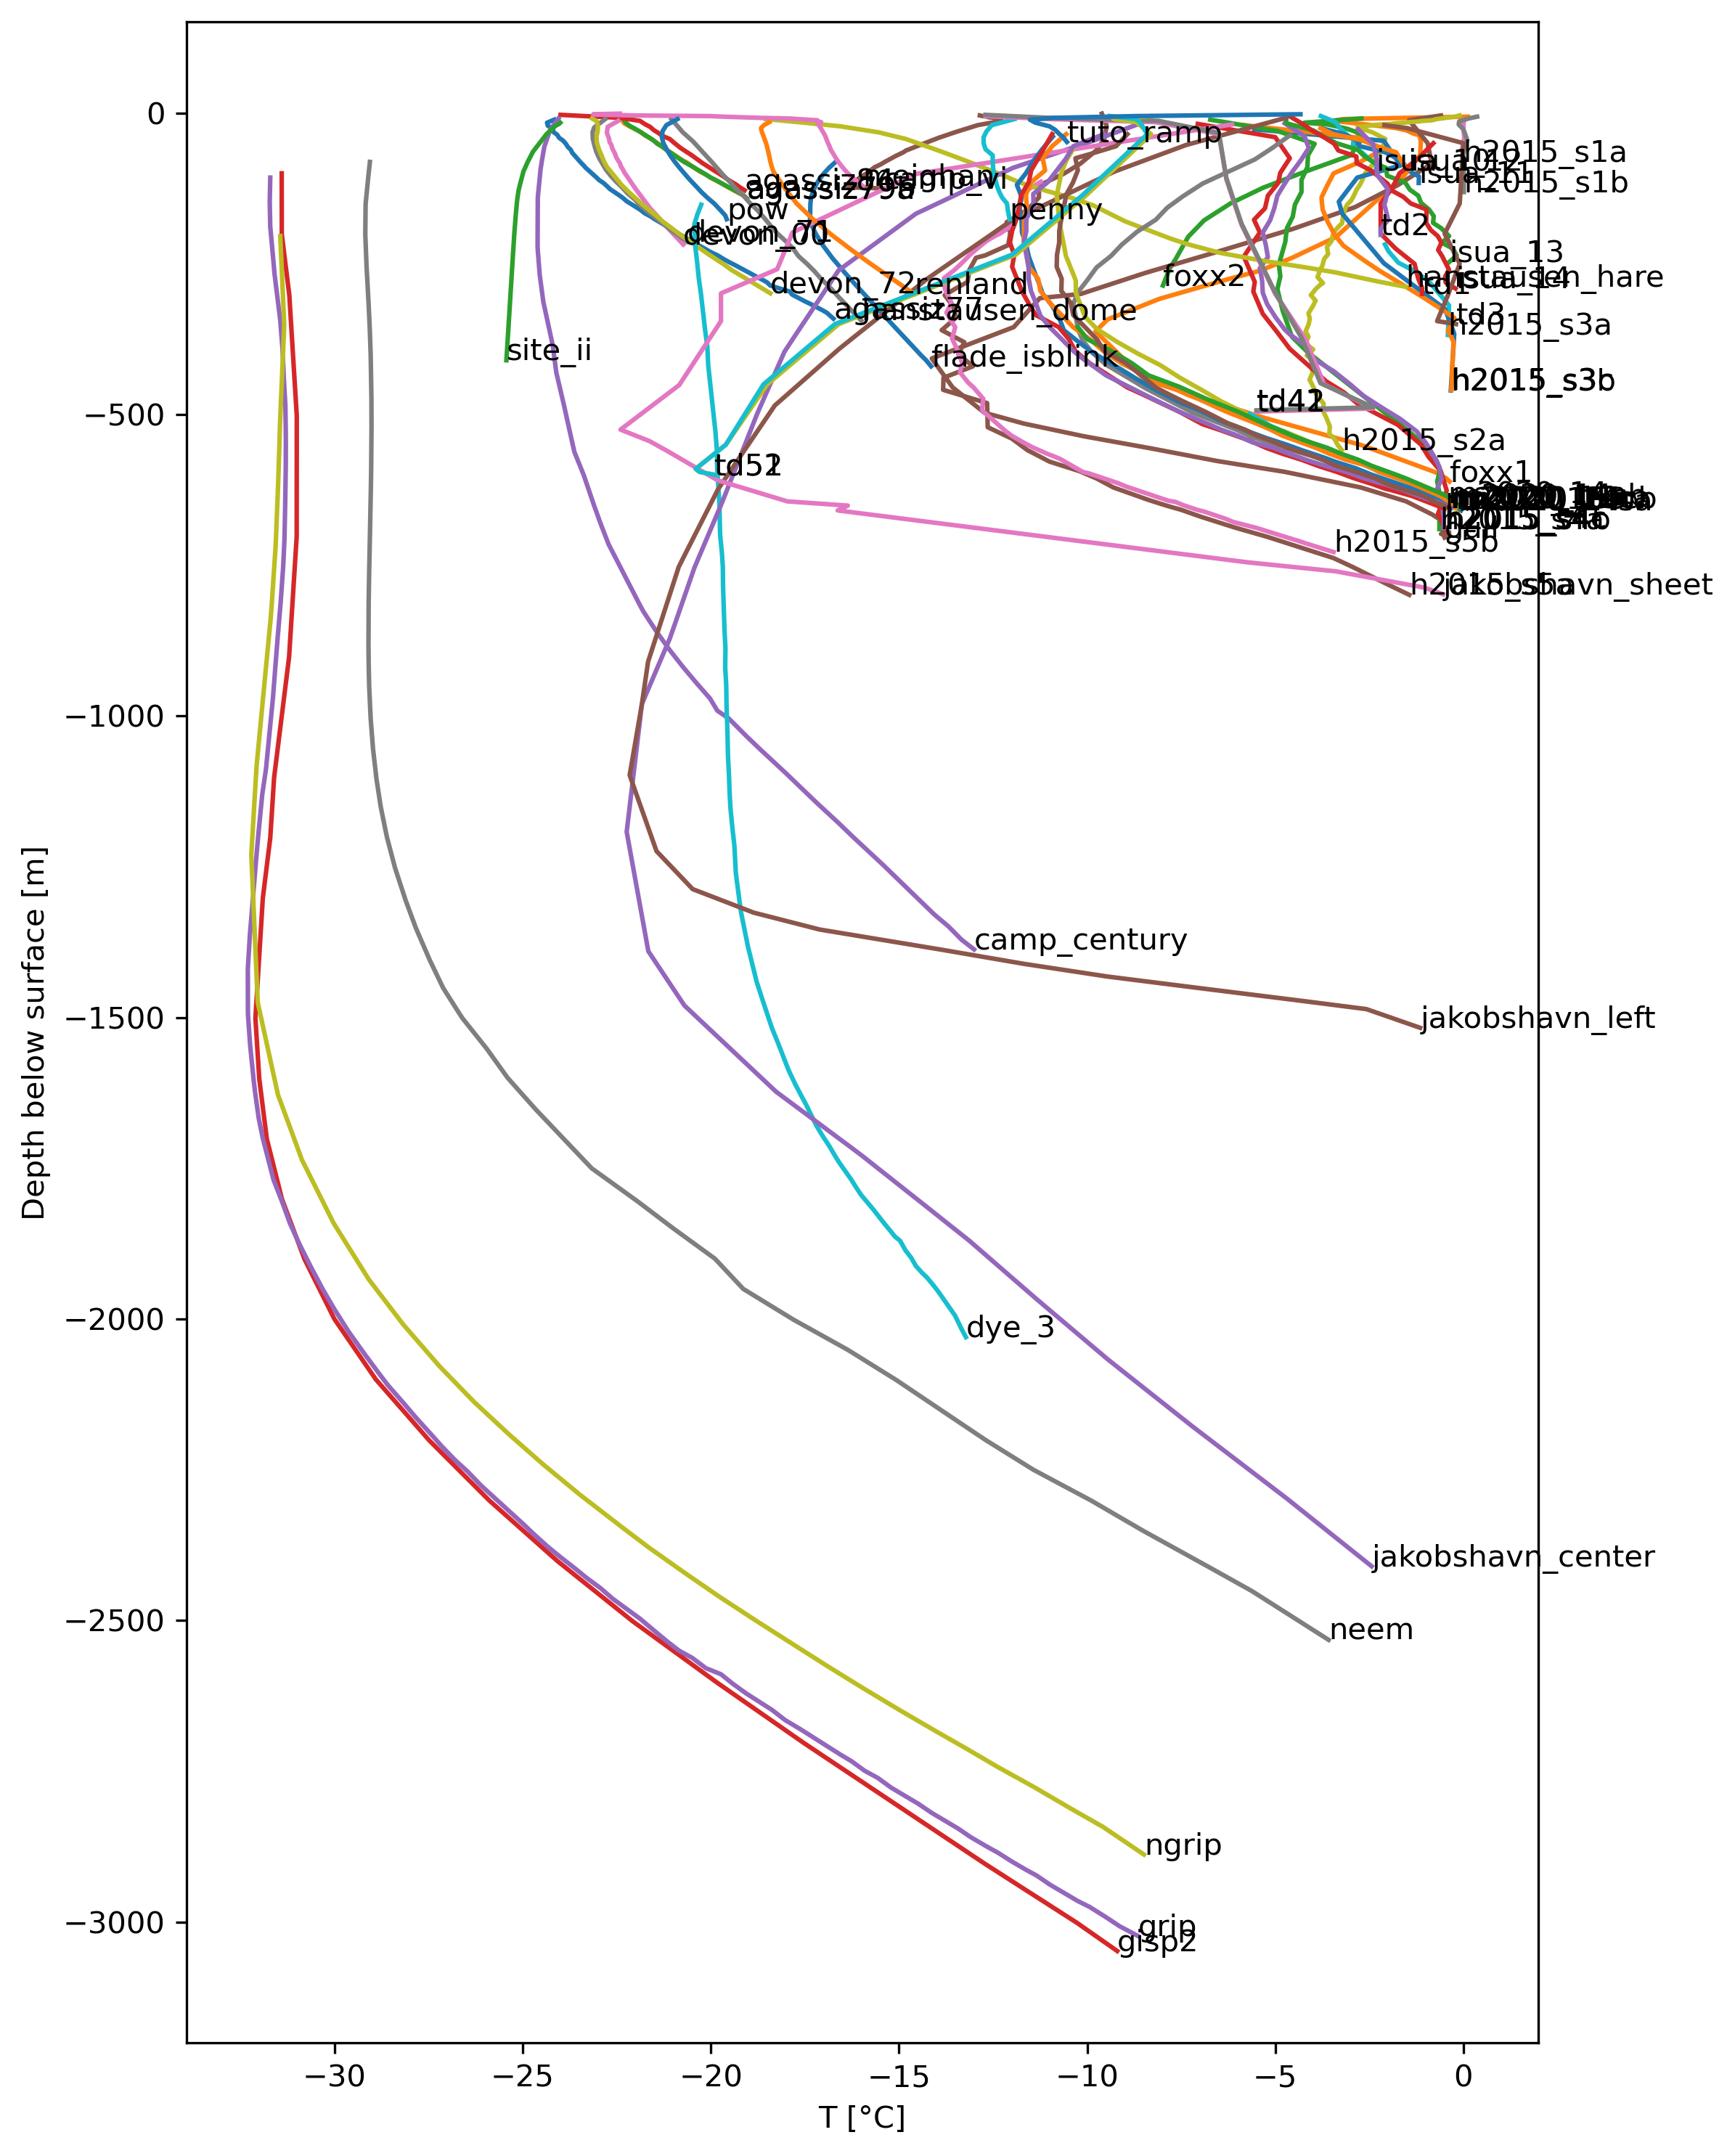
\includegraphics[width=.9\linewidth]{./T_surf.png}
\caption{\label{fig:T_surf}Temperature profiles from the surface}
\end{figure}

\begin{figure}[!h]
\centering
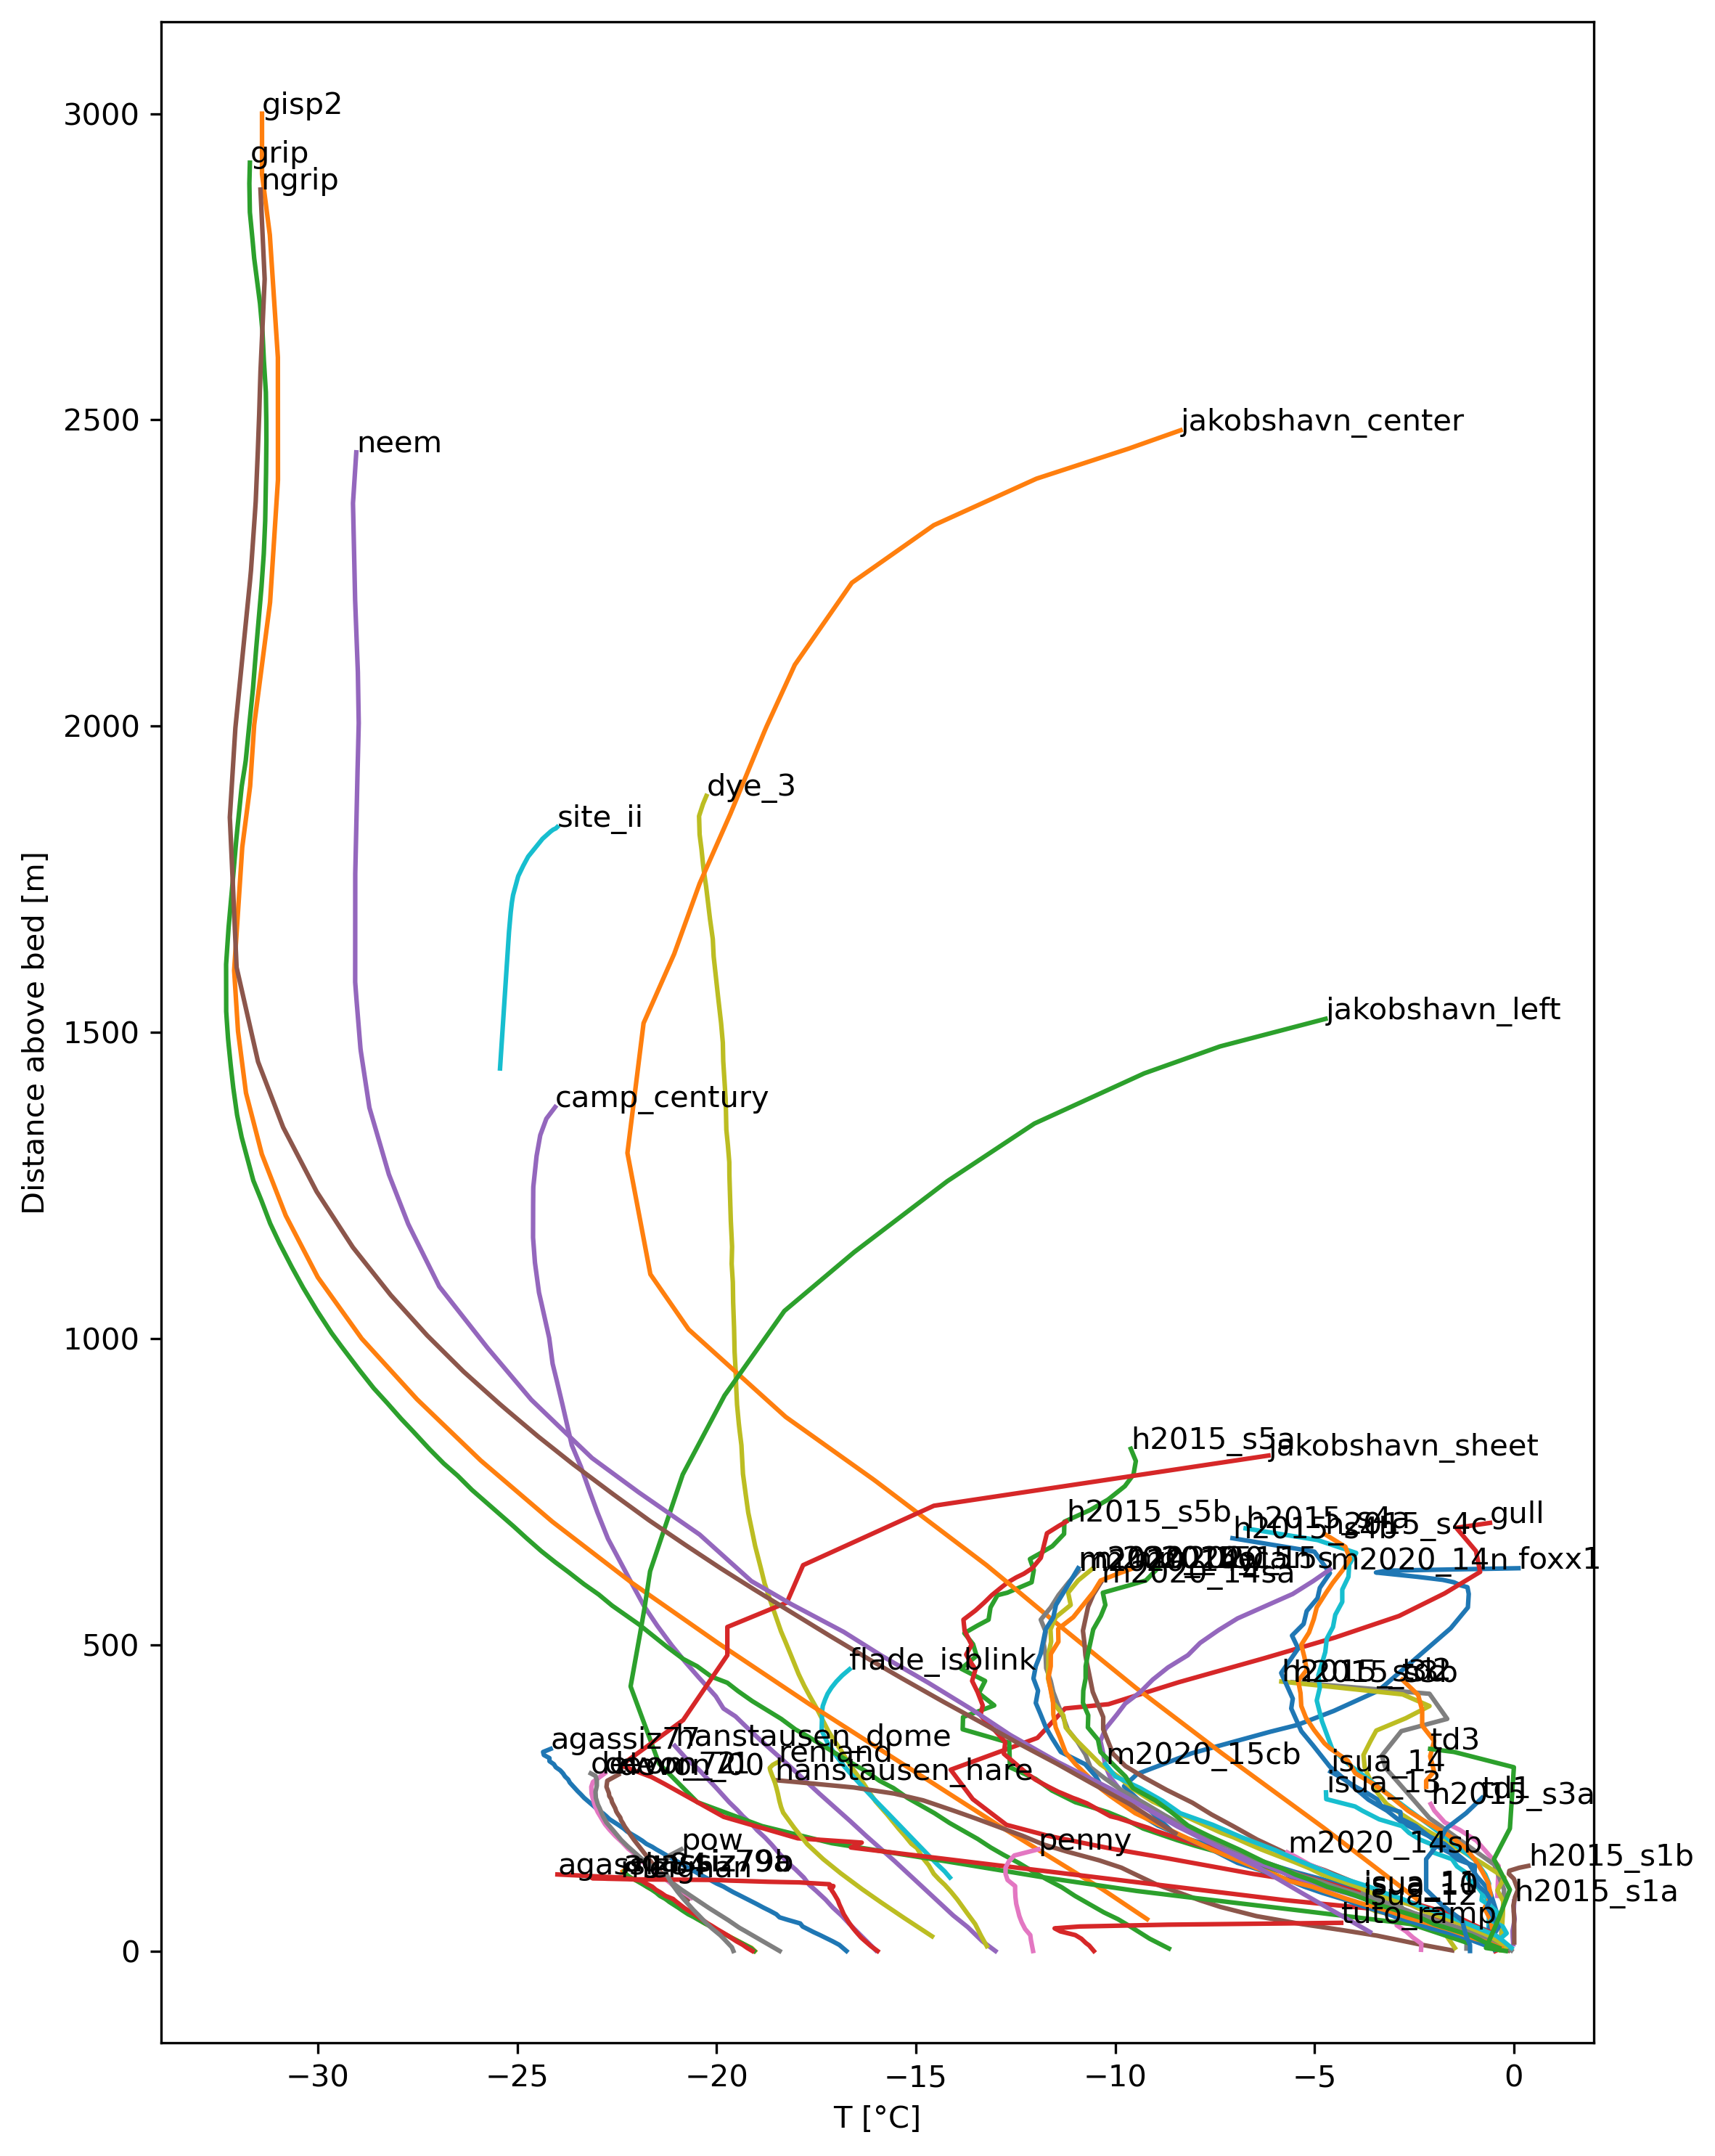
\includegraphics[width=.9\linewidth]{./T_bed.png}
\caption{\label{fig:T_bed}Temperature profiles from the bed}
\end{figure}

\begin{figure}[!h]
\centering
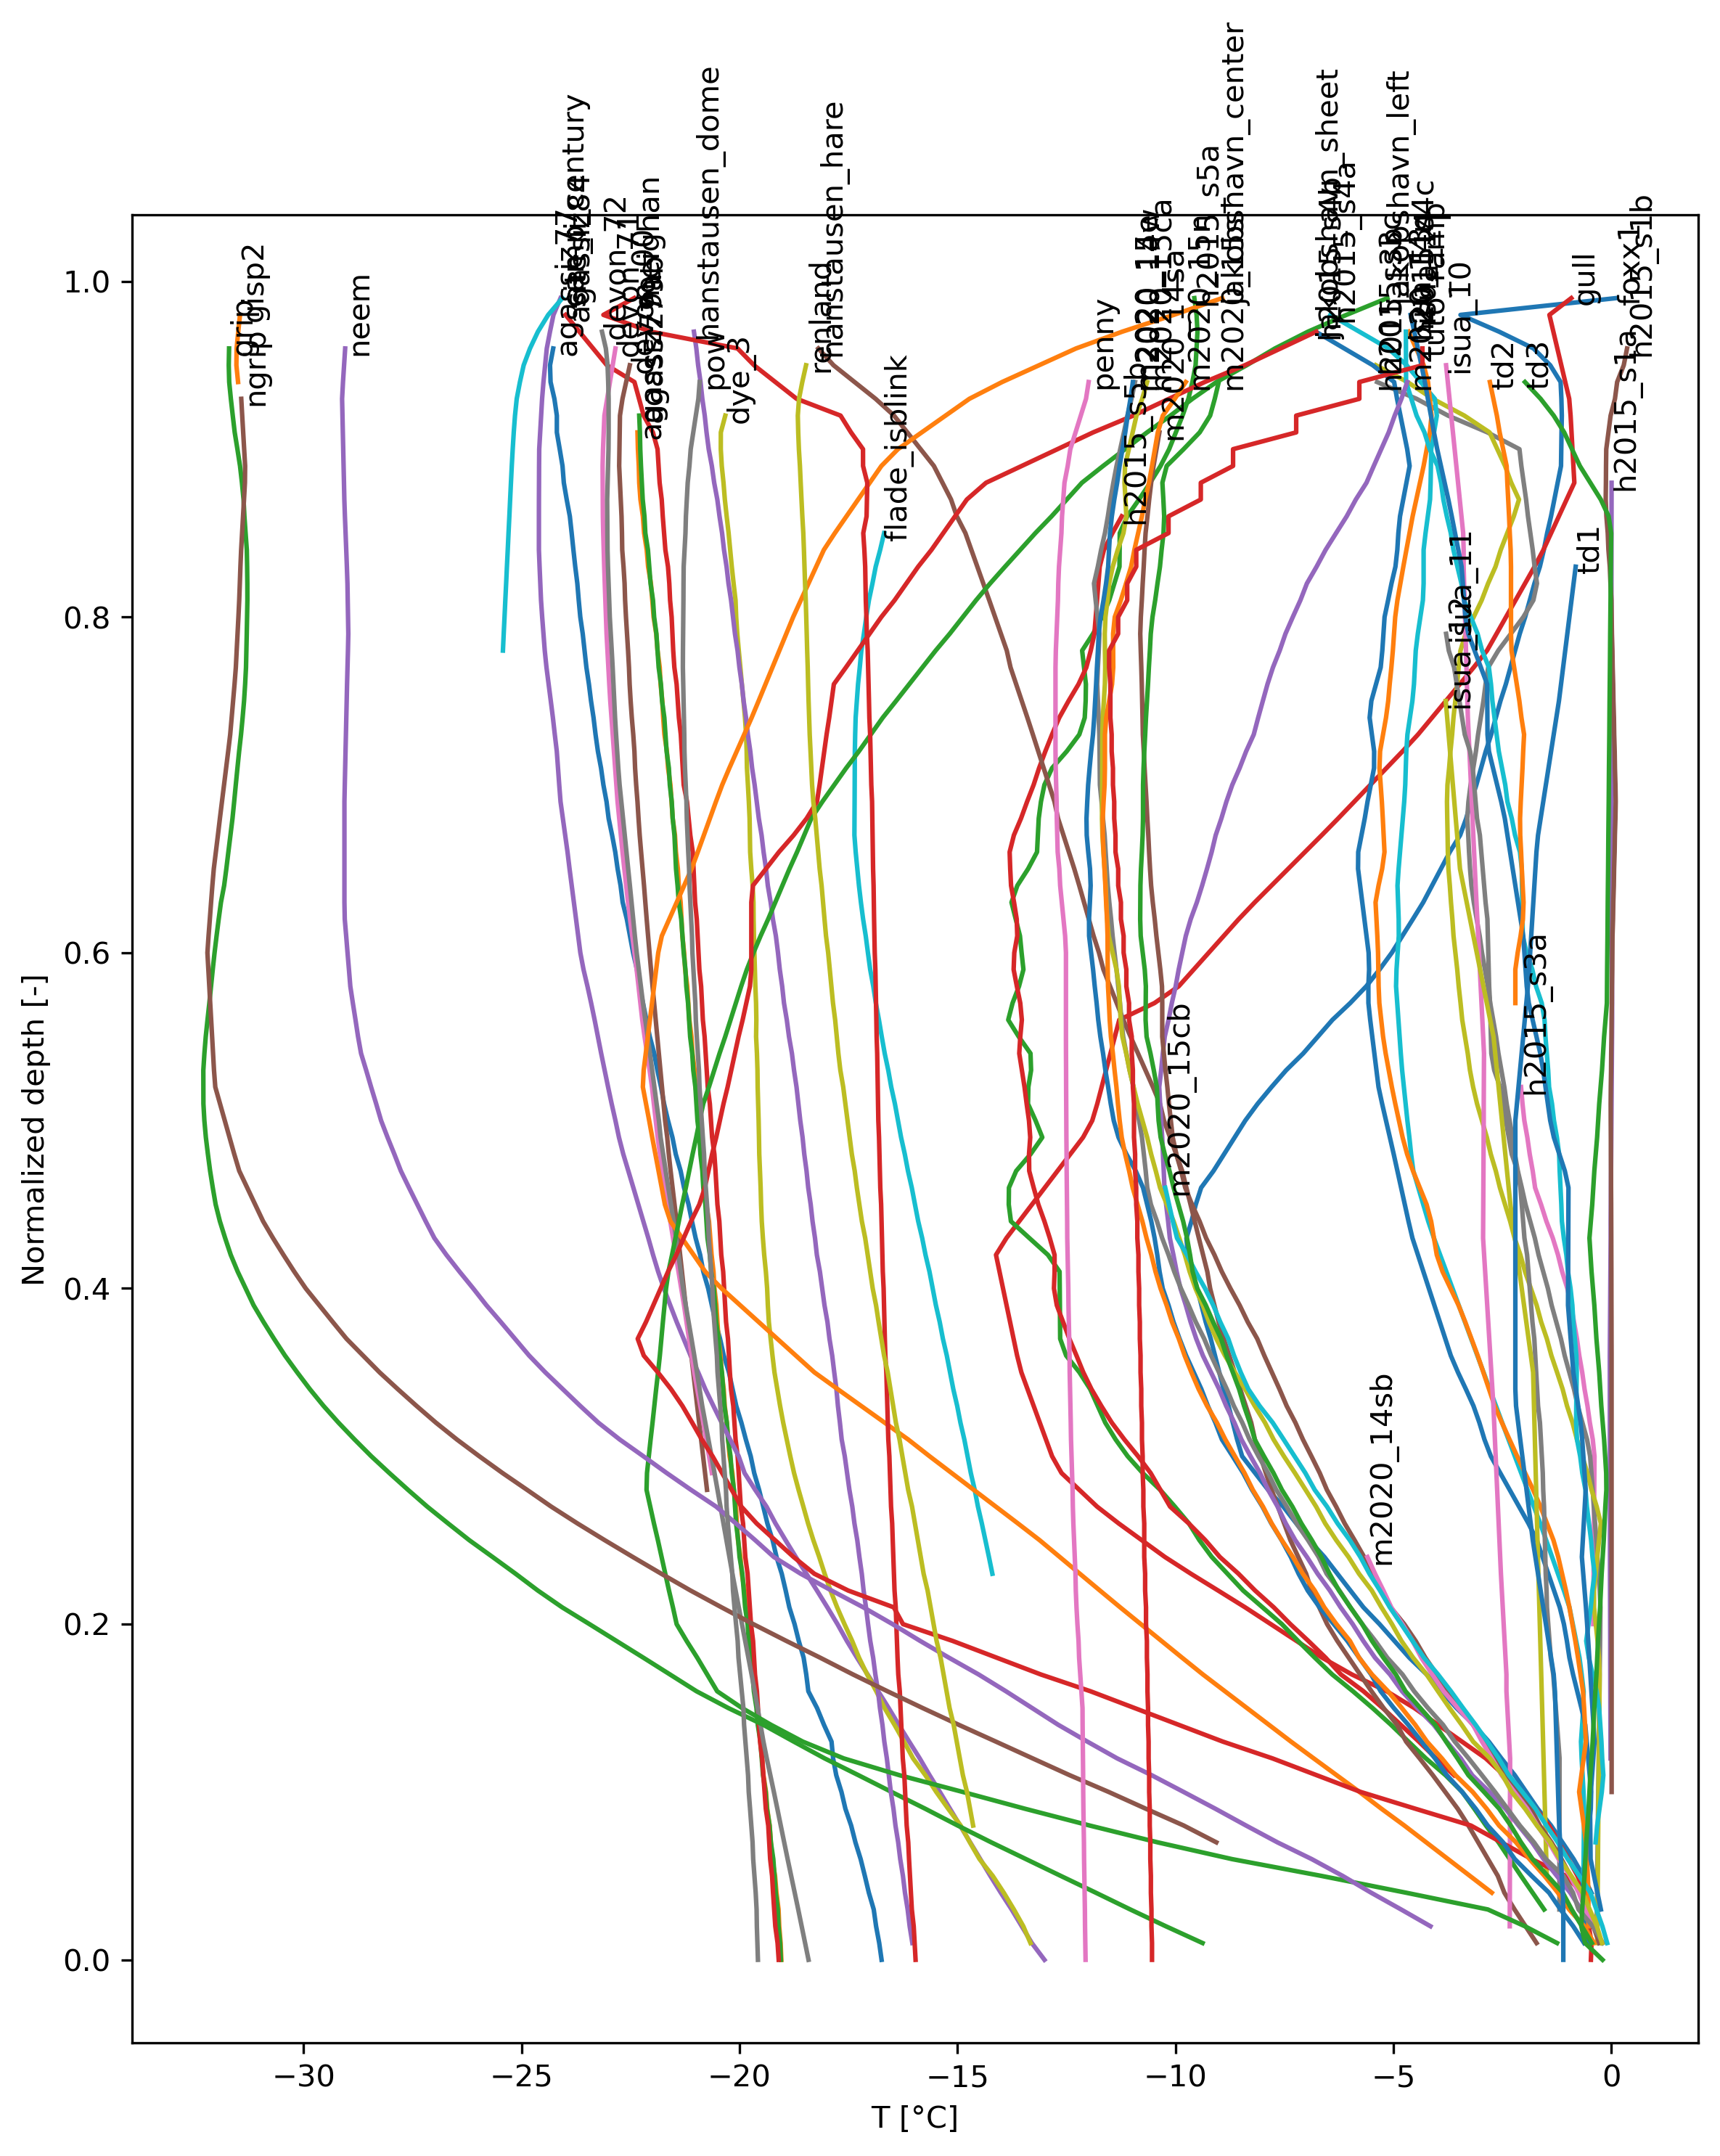
\includegraphics[width=.9\linewidth]{./T_norm.png}
\caption{\label{fig:T_norm}Temperature profiles from the surface (normalized depth)}
\end{figure}

\clearpage
\section{Source Material}
\label{sec:org17ccb2d}
\subsection{Agassiz 77 borehole}
\label{sec:orgcb37349}
\begin{verbatim}
Name                                  | agassiz77
Alternate name                        | Agassiz 77 borehole 
Data source                           | WIC Email
Data year(s)                          | 1977
Depth of top measurement [m]          | 11.0 
Depth of bottom measurement [m]       | 341.0 
Drill year(s)                         | 1977 (Vinther, 2008)
Longitude [°E]                        | -73.1 
Latitude [°N]                         | 80.7 
Approximate location name             | Agassiz Ice Cap 
Location source                       | Vinther, 2008
Ice thickness [m]                     | 340.9 
Ice thickness year                    | 
Ice thickness source                  | See data source 
Surface velocity [m yr^-1]            | 
Surface velocity year                 | 
Surface velocity source               | 
Measured from: Top, Bottom, Relative  | T 
\end{verbatim}

\subsubsection{Temperature}
\label{sec:orga89b6c4}

\begin{itemize}
\item Data provided by 3rd party in XLSX format, converted to CSV.
\item WIC Email: \href{msgid:AM0PR04MB6129DE88C9253A951702EE06A2F30@AM0PR04MB6129.eurprd04.prod.outlook.com}{Agassiz x4}
\item See also \textcite{clarke_1987_wind} Figure 2.
\end{itemize}

\begin{verbatim}
From: William Colgan
To: Ken Mankoff
Subject: Agassiz x4
Date: Wed 02 Dec 2020 04:54:17 AM PST
Attachments: [1]Agassiz borehole T profiles.xlsx(19.6K)

Here are 4x Agassiz Ice Cap temperature profiles. All to bedrock, and
all from within 2 km of the same 80.70N and 73.10W coordinate in the
file.

Fra: Christian Zdanowicz
Sendt: 2. december 2020 13:27
Til: William Colgan <wic@geus.dk>
Emne: RE: Prince of Wales - ice temperature?

The Agassiz T profiles are from the 1977, 1979 and 1984 boreholes, all
down to bedrock. I do not have more precise information on the
measurements or on the location of the boreholes than what was
published (see other attached papers).

David Fisher deserves the credit for all these data, I did not
generate them. You can use his Univ. of Ottawa affiliation: Department
of Earth and Environmental Sciences, University of Ottawa, Ottawa,
Canada, K1N 6N5.
\end{verbatim}

\subsubsection{Thickness}
\label{sec:org1570789}

From email (above) stating that profile goes to bedrock.

\subsubsection{Location}
\label{sec:org227a921}

Provided in email. Note: "within 2 km of".

\subsubsection{Velocity}
\label{sec:orgbb845b7}

Unknown
\clearpage
\subsection{Agassiz 79a borehole}
\label{sec:orgdcc0900}
\begin{verbatim}
Name                                  | agassiz79a
Alternate name                        | Agassiz ice cap 1979A borehole 
Data source                           | WIC Email 
Drill year(s)                         | 1979 (Vinther, 2008)
Data year(s)                          | 1979 
Longitude [°E]                        | -73.1 
Latitude [°N]                         | 80.7 
Approximate location name             | Agassiz Ice Cap 
Location source                       | Vinther, 2008
Ice thickness [m]                     | 141.9 
Ice thickness year                    | nan 
Ice thickness source                  | See data source 
Surface velocity [m yr^-1]            | nan 
Surface velocity year                 | nan 
Surface velocity source               | nan 
Measured from: Top, Bottom, Relative  | T 
Depth of top measurement [m]          | 12.0 
Depth of bottom measurement [m]       | 142.0 
Coverage [% of thickness]             | 92 
\end{verbatim}


\subsubsection{Temperature}
\label{sec:orgf6d748c}

\begin{itemize}
\item Data provided by 3rd party in XLSX format, converted to CSV.
\item WIC Email: \href{msgid:AM0PR04MB6129DE88C9253A951702EE06A2F30@AM0PR04MB6129.eurprd04.prod.outlook.com}{Agassiz x4}
\item See also \textcite{clarke_1987_wind} Figure 2.
\end{itemize}

\begin{verbatim}
From: William Colgan
To: Ken Mankoff
Subject: Agassiz x4
Date: Wed 02 Dec 2020 04:54:17 AM PST
Attachments: [1]Agassiz borehole T profiles.xlsx(19.6K)

Here are 4x Agassiz Ice Cap temperature profiles. All to bedrock, and
all from within 2 km of the same 80.70N and 73.10W coordinate in the
file.

Fra: Christian Zdanowicz
Sendt: 2. december 2020 13:27
Til: William Colgan <wic@geus.dk>
Emne: RE: Prince of Wales - ice temperature?

The Agassiz T profiles are from the 1977, 1979 and 1984 boreholes, all
down to bedrock. I do not have more precise information on the
measurements or on the location of the boreholes than what was
published (see other attached papers).

David Fisher deserves the credit for all these data, I did not
generate them. You can use his Univ. of Ottawa affiliation: Department
of Earth and Environmental Sciences, University of Ottawa, Ottawa,
Canada, K1N 6N5.
\end{verbatim}

\subsubsection{Thickness}
\label{sec:org78d23e7}

From email (above) stating that profile goes to bedrock.

\subsubsection{Location}
\label{sec:org609731a}

Provided in email. Note: "within 2 km of".

\subsubsection{Velocity}
\label{sec:org3e40b3f}

Unknown
\clearpage
\subsection{Agassiz 79b borehole}
\label{sec:org8f041f9}
\begin{verbatim}
Name                                  | agassiz79b
Alternate name                        | Agassiz ice cap 1979B borehole
Data source                           | WIC Email
Drill year(s)                         | 1979 (Vinther, 2008)
Data year(s)                          | 1979
Longitude [°E]                        | -73.1
Latitude [°N]                         | 80.7
Approximate location name             | Agassiz Ice Cap
Location source                       | Vinther (2008)
Ice thickness [m]                     | 141.2
Ice thickness year                    | nan
Ice thickness source                  | See data source
Surface velocity [m yr^-1]            | nan
Surface velocity year                 | nan
Surface velocity source               | nan
Measured from: Top, Bottom, Relative  | T
Depth of top measurement [m]          | 11.0
Depth of bottom measurement [m]       | 141.0
Coverage [% of thickness]             | 92
\end{verbatim}

\subsubsection{Temperature}
\label{sec:org068e2a1}

\begin{itemize}
\item Data provided by 3rd party in XLSX format, converted to CSV.
\item WIC Email: \href{msgid:AM0PR04MB6129DE88C9253A951702EE06A2F30@AM0PR04MB6129.eurprd04.prod.outlook.com}{Agassiz x4}
\item See also \textcite{clarke_1987_wind} Figure 2.
\end{itemize}

\begin{verbatim}
From: William Colgan
To: Ken Mankoff
Subject: Agassiz x4
Date: Wed 02 Dec 2020 04:54:17 AM PST
Attachments: [1]Agassiz borehole T profiles.xlsx(19.6K)

Here are 4x Agassiz Ice Cap temperature profiles. All to bedrock, and
all from within 2 km of the same 80.70N and 73.10W coordinate in the
file.

Fra: Christian Zdanowicz
Sendt: 2. december 2020 13:27
Til: William Colgan <wic@geus.dk>
Emne: RE: Prince of Wales - ice temperature?

The Agassiz T profiles are from the 1977, 1979 and 1984 boreholes, all
down to bedrock. I do not have more precise information on the
measurements or on the location of the boreholes than what was
published (see other attached papers).

David Fisher deserves the credit for all these data, I did not
generate them. You can use his Univ. of Ottawa affiliation: Department
of Earth and Environmental Sciences, University of Ottawa, Ottawa,
Canada, K1N 6N5.
\end{verbatim}

\subsubsection{Thickness}
\label{sec:org04b53b1}

From email (above) stating that profile goes to bedrock.

\subsubsection{Location}
\label{sec:org0baeb48}

Provided in email. Note: "within 2 km of".

\subsubsection{Velocity}
\label{sec:org5abab91}

Unknown
\clearpage
\subsection{Agassiz 84 borehole}
\label{sec:org4eaf90f}
\begin{verbatim}
Name                                  | agassiz84
Alternate name                        | Agassiz 1984 borehole
Data source                           | WIC Email
Drill year(s)                         | 184 (Vinther, 2008)
Data year(s)                          | 1984
Longitude [°E]                        | -73.1
Latitude [°N]                         | 80.7
Approximate location name             | Agassiz Ice Cap
Location source                       | Vinther, 2008
Ice thickness [m]                     | 127.6
Ice thickness year                    | nan
Ice thickness source                  | See data source
Surface velocity [m yr^-1]            | nan
Surface velocity year                 | nan
Surface velocity source               | nan
Measured from: Top, Bottom, Relative  | T
Depth of top measurement [m]          | 3.0
Depth of bottom measurement [m]       | 128.0
Coverage [% of thickness]             | 98
\end{verbatim}

\subsubsection{Temperature}
\label{sec:org824a6ed}

\begin{itemize}
\item Data provided by 3rd party in XLSX format, converted to CSV.
\item WIC Email: \href{msgid:AM0PR04MB6129DE88C9253A951702EE06A2F30@AM0PR04MB6129.eurprd04.prod.outlook.com}{Agassiz x4}
\item See also \textcite{clarke_1987_wind} Figure 2.
\end{itemize}

\begin{verbatim}
From: William Colgan
To: Ken Mankoff
Subject: Agassiz x4
Date: Wed 02 Dec 2020 04:54:17 AM PST
Attachments: [1]Agassiz borehole T profiles.xlsx(19.6K)

Here are 4x Agassiz Ice Cap temperature profiles. All to bedrock, and
all from within 2 km of the same 80.70N and 73.10W coordinate in the
file.

Fra: Christian Zdanowicz
Sendt: 2. december 2020 13:27
Til: William Colgan <wic@geus.dk>
Emne: RE: Prince of Wales - ice temperature?

The Agassiz T profiles are from the 1977, 1979 and 1984 boreholes, all
down to bedrock. I do not have more precise information on the
measurements or on the location of the boreholes than what was
published (see other attached papers).

David Fisher deserves the credit for all these data, I did not
generate them. You can use his Univ. of Ottawa affiliation: Department
of Earth and Environmental Sciences, University of Ottawa, Ottawa,
Canada, K1N 6N5.
\end{verbatim}

\subsubsection{Thickness}
\label{sec:org7189fdc}

From email (above) stating that profile goes to bedrock.

\subsubsection{Location}
\label{sec:org160c109}

Provided in email. Note: "within 2 km of".

\subsubsection{Velocity}
\label{sec:org60b3e9d}

Unknown
\clearpage
\subsection{Camp Century}
\label{sec:org70bfc24}
\begin{verbatim}
Name                                  | camp_century
Alternate name                        | Camp Century
Data source                           | Weertman, J.: Comparison betwe
Drill year(s)                         | nan
Data year(s)                          | nan
Longitude [°E]                        | nan
Latitude [°N]                         | nan
Approximate location name             | Camp Century
Location source                       | ?
Ice thickness [m]                     | 1387
ice thickness year                    | ?
Ice thickness source                  | ?
Surface velocity [m yr^-1]            | nan
Surface velocity year                 | nan
Surface velocity source               | nan
Measured from: Top, Bottom, Relative  | B
Depth of top measurement [m]          | 9.0
Depth of bottom measurement [m]       | 1387.0
Coverage [% of thickness]             | 99
\end{verbatim}

\subsubsection{Temperature}
\label{sec:org729292c}

\begin{itemize}
\item Digitized from \textcite{weertman_1968} Figure 1
\item Note: Temperature depth scale is from bottom.
\item Note (from Liam Colgan): \textcite{weertman_1968} shows \textasciitilde{} -12 °C at the bed in 1966, but a small ensemble of radar analyses now show liquid bed returns since 2010.
\end{itemize}


\begin{center}
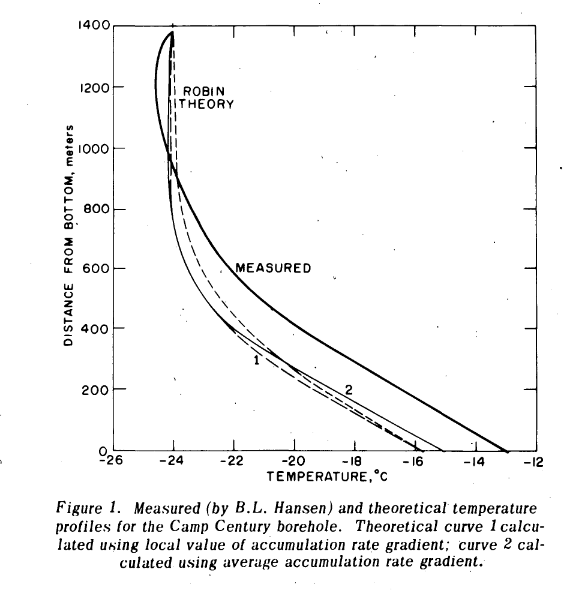
\includegraphics[width=.9\linewidth]{camp_century/weertman_1968_fig1.png}
\end{center}

\subsubsection{Thickness}
\label{sec:orgf5157a5}

Unknown source - check with WIC

\subsubsection{Location}
\label{sec:orgc44a740}

Unknown

\subsubsection{Velocity}
\label{sec:org491c6e0}

Unknown
\clearpage
\subsection{Devon 1998/2000 borehole}
\label{sec:org1b641fa}
\begin{verbatim}
Name                                  | devon_00
Alternate name                        | Devon borehole
Data source                           | WIC Email
Drill year(s)                         | 1998-04-15 to 1998-05-07
Data year(s)                          | 2000-04-15
Longitude [°E]                        | -82.14
Latitude [°N]                         | 75.34
Approximate location name             | Devon Ice Cap
Location source                       | 
Ice thickness [m]                     | 300.55
ice thickness year                    | 
Ice thickness source                  | See data source
Surface velocity [m yr^-1]            | 
Surface velocity year                 | 
Surface velocity source               | 
Measured from: Top, Bottom, Relative  | T
Depth of top measurement [m]          | 13
Depth of bottom measurement [m]       | 218
\end{verbatim}

\subsubsection{Temperature}
\label{sec:org1b63cbd}

\begin{itemize}
\item Provided in XLSX file via email.
\begin{itemize}
\item Link to email: \href{msgid:AM0PR04MB61295B7BB1FF4BE1112B94ABA2F30@AM0PR04MB6129.eurprd04.prod.outlook.com}{VS: Prince of Wales - ice temperature?}
\end{itemize}
\item Note that temperature profile starts at casement, 1.55 m below Y2K surface, so all depths have +1.55 added to them.
\end{itemize}

\begin{verbatim}
From: William Colgan
To: Ken Mankoff
Subject: VS: Prince of Wales - ice temperature?
Date: Wed 02 Dec 2020 03:10:34 AM PST
Attachments: [1]Devon 1998 borehole Ts.xlsx(12.1K)

Ken – Devon98 temperature profile. Goes down to 217 m, bed at 299m.
Coordinates: N 75 deg 20.40, W 82 deg 08.40

Fra: Christian Zdanowicz
Sendt: 2. december 2020 11:39
Til: William Colgan
Emne: RE: Prince of Wales - ice temperature?

Re: Devon ice cap 1998

N 75 deg 20.40, W 82 deg 08.40
Alt: 1930 m asl

See Fig. 1 of attached paper for exact location.

David Fisher did the measurements using a thermistor string. [...] I
may have given you false hopes on this one, because the temperatures
on the deepest part of the borehole are sadly missing: David's notes
say the cable broke at 216 m depth ! The bottom of the hole was at 299
m. You could take a shot at extrapolating the gradient, of course,
maybe it agrees with the 72 and 73 boreholes.
\end{verbatim}

\subsubsection{Thickness}
\label{sec:org0395013}

\begin{itemize}
\item Reported in email, also adjusted by 1.55 m.
\end{itemize}

\subsubsection{Location}
\label{sec:org24eed79}

\begin{itemize}
\item Reported in email
\end{itemize}

\subsubsection{Velocity}
\label{sec:org9ec8aa8}
\clearpage
\subsection{Devon 1971 borehole}
\label{sec:orgbc33dd5}
\begin{verbatim}
Name                                  | devon_71
Alternate name                        | Devon borehole
Data source                           | Paterson, W. S. B., Clarke, G. K. C.: Comparison of theoretical and observed temperature profiles in Devon Island ice cap, Canada , Geophysical Journal International 55(3), Oxford University Press (OUP), 615–632, 12 1978 
Drill year(s)                         | 
Data year(s)                          | 
Longitude [°E]                        | 
Latitude [°N]                         | 
Approximate location name             | Devon Ice Cap
Location source                       | 
Ice thickness [m]                     | 300
ice thickness year                    | drill year
Ice thickness source                  | See data source
Surface velocity [m yr^-1]            | 
Surface velocity year                 | 
Surface velocity source               | 
Measured from: Top, Bottom, Relative  | T
Depth of top measurement [m]          | 10
Depth of bottom measurement [m]       | 213
\end{verbatim}

\subsubsection{Temperature}
\label{sec:org0336ee2}

Digitized from \textcite{paterson_1978} Figure 2a.

\begin{center}
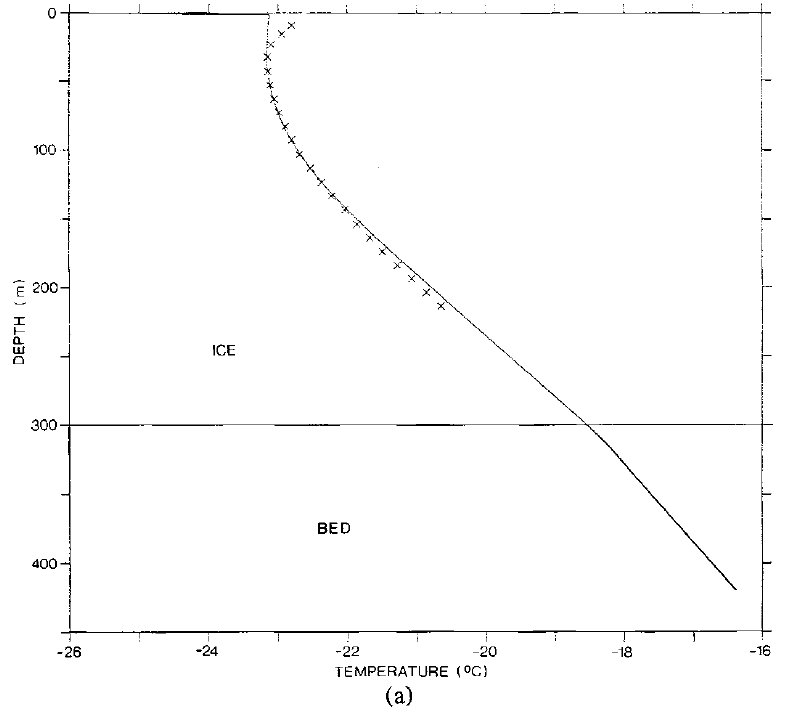
\includegraphics[width=.9\linewidth]{devon_71/paterson_1978_fig2a.png}
\end{center}

\subsubsection{Thickness}
\label{sec:org2bad5f1}

Provided by in graphics and text.

\subsubsection{Location}
\label{sec:org0bd87af}

Can probably be extracted from Figure 1

\begin{center}
\includegraphics[width=.9\linewidth]{devon_71/paterson_1978_fig1.png}
\end{center}

\subsubsection{Velocity}
\label{sec:org9ea9af9}

Unknown
\clearpage
\subsection{Devon 1972 borehole}
\label{sec:org15ddc24}
\begin{verbatim}
Name                                  | devon_72
Alternate name                        | Devon borehole
Data source                           | Paterson, W. S. B., Clarke, G. K. C.: Comparison of theoretical and observed temperature profiles in Devon Island ice cap, Canada , Geophysical Journal International 55(3), Oxford University Press (OUP), 615–632, 12 1978 
Drill year(s)                         | 
Data year(s)                          | 
Longitude [°E]                        | -82.14
Latitude [°N]                         | 75.34
Approximate location name             | Devon Ice Cap
Location source                       | 
Ice thickness [m]                     | 299
ice thickness year                    | drill year
Ice thickness source                  | See data source
Surface velocity [m yr^-1]            | 
Surface velocity year                 | 
Surface velocity source               | 
Measured from: Top, Bottom, Relative  | T
Depth of top measurement [m]          | 9
Depth of bottom measurement [m]       | 299
\end{verbatim}


\subsubsection{Temperature}
\label{sec:org1589a66}

Digitized from \textcite{paterson_1978} Figure 2b.

\begin{center}
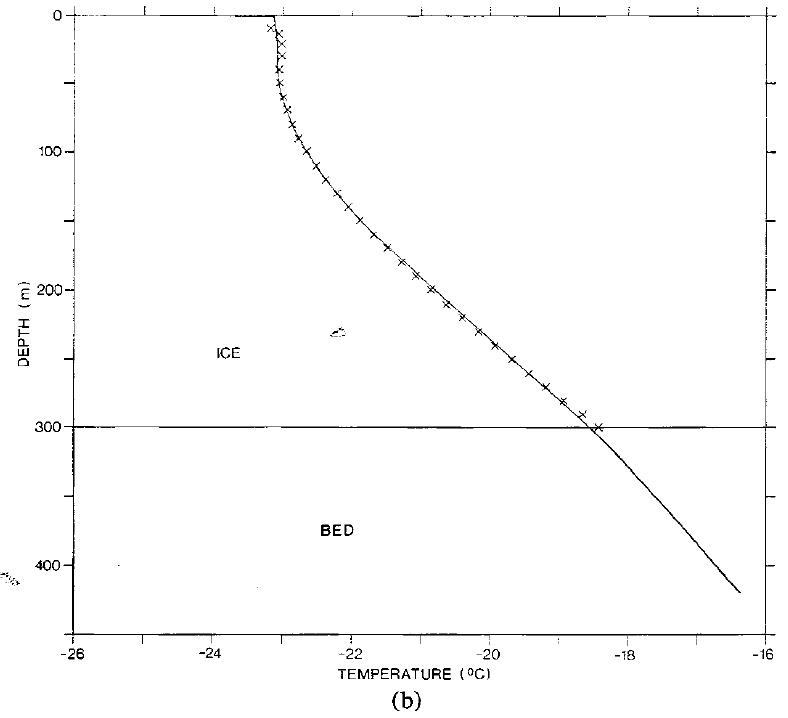
\includegraphics[width=.9\linewidth]{devon_72/paterson_1978_fig2b.png}
\end{center}

\subsubsection{Thickness}
\label{sec:org8ae1cf9}

Provided by \textcite{paterson_1978} in graphics and text.

\subsubsection{Location}
\label{sec:orgc1621d8}

Can probably be extracted from \textcite{paterson_1978} Figure 1

\begin{center}
\includegraphics[width=.9\linewidth]{devon_72/paterson_1978_fig1.png}
\end{center}

\subsubsection{Velocity}
\label{sec:org6c03f85}

Unknown
\clearpage
\subsection{DYE-3}
\label{sec:org31b8c7b}
\begin{verbatim}
Name                                  | dye_3
Alternate name                        | DYE-3
Data source                           | Gundestrup, N. S., Hansen, B. Lyle: Bore-Hole Survey at Dye 3, South Greenland , Journal of Glaciology 30(106), Cambridge University Press (CUP), 282–288, 1984 
Drill year(s)                         | 1979 to 1981
Data year(s)                          | 1983
Longitude [°E]                        | -43.816667
Latitude [°N]                         | 65.183333
Approximate location name             | South Greenland
Location source                       | See data source
Ice thickness [m]                     | 2038
ice thickness year                    | 1983
Ice thickness source                  | See data source
Surface velocity [m yr^-1]            | 
Surface velocity year                 | 
Surface velocity source               | 
Measured from: Top, Bottom, Relative  | T
Depth of top measurement [m]          | 152
Depth of bottom measurement [m]       | 2030
\end{verbatim}

\subsubsection{Temperature}
\label{sec:org813ba08}

Digitized from \textcite{gundestrup_1984} Figure 4.

We only use 1983 profile digitized with the bottom x-axis.

The 1980 and 1982 profiles use the top x-axis (expanded temperature scale).

\begin{center}
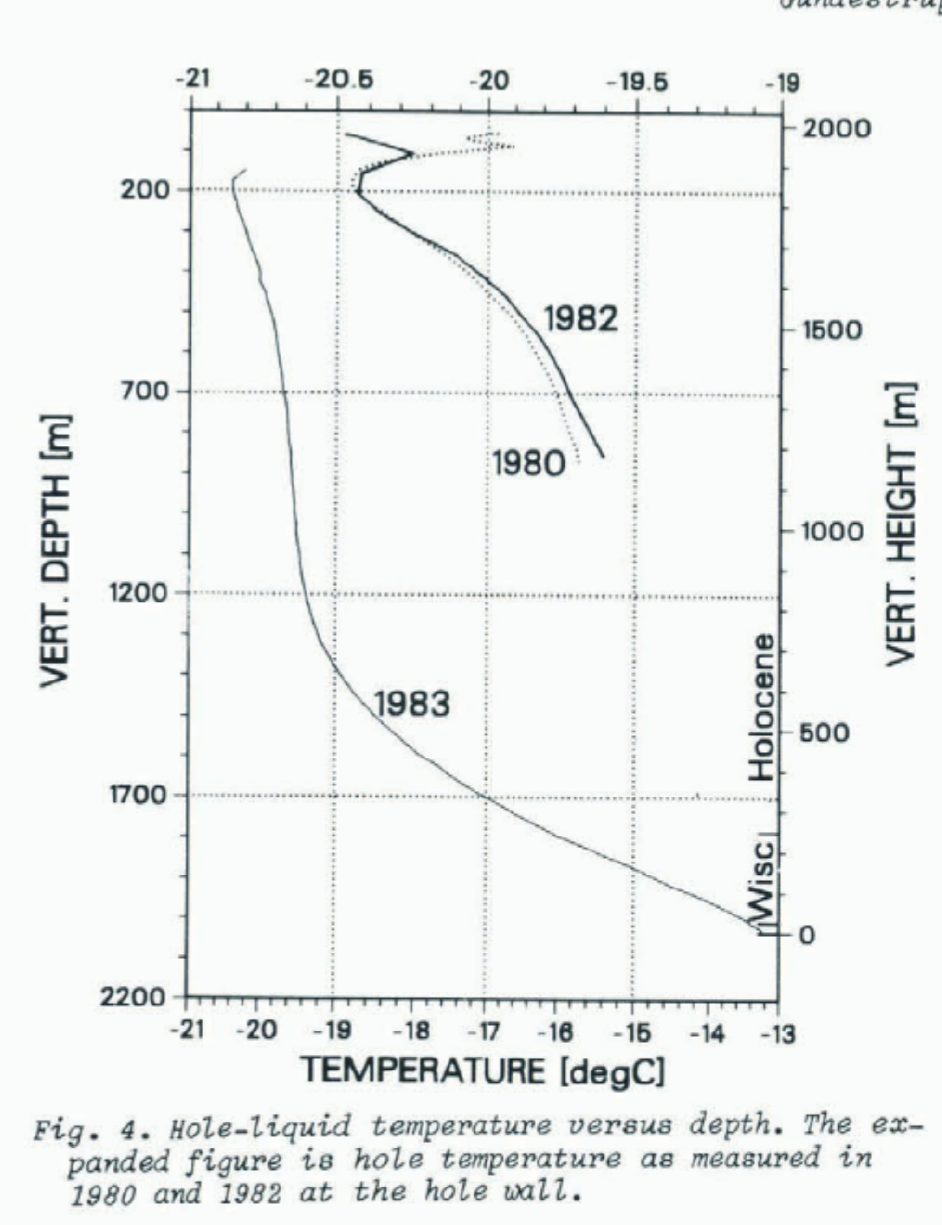
\includegraphics[width=.9\linewidth]{dye_3/gundestrup_1984_fig4.png}
\end{center}

\subsubsection{Thickness}
\label{sec:org71544f4}

Reported in \textcite{gundestrup_1984} from graphic.

\subsubsection{Location}
\label{sec:org25290f6}

Reported in \textcite{gundestrup_1984}.

\subsubsection{Velocity}
\label{sec:org818ad35}
\clearpage
\subsection{Flade Isblink}
\label{sec:orga526daf}
\begin{verbatim}
Name                                  | flade_isblink
Alternate name                        | Flade Isblink
Data source                           | Dorthe Dalh-Jensen (personal comm.)
Drill year(s)                         | 
Data year(s)                          | 
Longitude [°E]                        | -15.7029
Latitude [°N]                         | 81.2926
Approximate location name             | 
Location source                       | 
Ice thickness [m]                     | 540
ice thickness year                    | 
Ice thickness source                  | See WIC email
Surface velocity [m yr^-1]            | 
Surface velocity year                 | 
Surface velocity source               | 
Measured from: Top, Bottom, Relative  | T
Depth of top measurement [m]          | 80.0
Depth of bottom measurement [m]       | 420.0
\end{verbatim}

\subsubsection{Temperature}
\label{sec:orgb7847a4}

\begin{itemize}
\item Provided by Dorthe Dahl-Jensen (personal comm.). See above.
\item Link to email: \href{msgid:AM0PR04MB61299127D5D5EF0A7269A855A2DF0@AM0PR04MB6129.eurprd04.prod.outlook.com}{VS: Greenland geothermal?}
\item It appears temperature was measured at some locations 2x, perhaps while lowering and raising a thermometer?
\end{itemize}

\begin{verbatim}
From: William Colgan
To: Ken Mankoff
Subject: VS: Greenland geothermal?
Date: Tue 22 Dec 2020 11:06:16 AM PST

  1.  Total depth: 540 m (borehole on reached 425m).
  2.  Temperature data below
  3.  Location: 81.2926 N -15.7029 E

Fra: Dorthe Dahl-Jensen
Sendt: 22. december 2020 16:17
Til: William Colgan; Bo Vinther
Emne: Re: Greenland geothermal?

Also for Flade Isblink (ref: Dahl-Jensen, personal com)

80      -16.664
90      -16.845
100     -16.994
110     -17.116
120     -17.214
130     -17.28
140     -17.335
150     -17.353
160     -17.356
420     -14.146
410     -14.277
400     -14.44
380     -14.737
360     -15.035
340     -15.333
320     -15.626
300     -15.93
280     -16.222
260     -16.505
240     -16.777
220     -17.013
200     -17.214
180     -17.364
160     -17.434
140     -17.385
120     -17.277
\end{verbatim}

\subsubsection{Thickness}
\label{sec:org710dd2e}

From WIC email

\subsubsection{Location}
\label{sec:orgc669546}

From WIC email

\subsubsection{Velocity}
\label{sec:orgf5cfd46}
\clearpage
\subsection{FOXX1}
\label{sec:orgc717d4d}
\begin{verbatim}
Name                                  | foxx1
Alternate name                        | FOXX
Data source                           | Lüthi, Martin P., Ryser, Claudia, Andrews, Lauren C., Catania, Ginny A., Funk, Martin, Hawley, Robert L., Hoffman, Matthew J., Neumann, Thomas A.: Heat sources within the Greenland Ice Sheet: dissipation, temperate paleo-firn and cryo-hydrologic warming , The Cryosphere 9(1), 245–253, 2015 
Drill year(s)                         | 
Data year(s)                          | 2011-2013
Longitude [°E]                        | -49° 53.107'
Latitude [°N]                         | 69° 26.755'
Approximate location name             | Paakitsoq
Location source                       | Ryser (2014) doi:10.1002/2013JF003067
Ice thickness [m]                     | 620
ice thickness year                    | 
Ice thickness source                  | Ryser (2014) doi:10.1002/2013JF003067
Surface velocity [m yr^-1]            | 
Surface velocity year                 | 
Surface velocity source               | 
Measured from: Top, Bottom, Relative  | T
Depth of top measurement [m]          | 105.0
Depth of bottom measurement [m]       | 624.0
\end{verbatim}

\subsubsection{Temperature}
\label{sec:org8a88e55}

\begin{itemize}
\item Digitized from \textcite{luthi_2015} Figure 2:
\end{itemize}

\begin{center}
\includegraphics[width=.9\linewidth]{foxx1/luthi_2015_fig2_all.png}
\end{center}

\subsubsection{Thickness}
\label{sec:org06a54d7}

\begin{itemize}
\item From \textcite{ryser_2014_caterpillar}.
\end{itemize}

\subsubsection{Location}
\label{sec:org172fe35}

\begin{itemize}
\item From \textcite{ryser_2014_caterpillar}.
\end{itemize}

\subsubsection{Velocity}
\label{sec:orgd70c78b}

\begin{itemize}
\item From \textcite{ryser_2014_caterpillar}.
\end{itemize}

\begin{quote}
Measured surface velocities of about 100 m a−1 are
modulated by seasonal velocity variations; winter
velocities of 70 to 80 m a−1 eventually double during
speedup events in summer. 
\end{quote}
\clearpage
\subsection{FOXX2}
\label{sec:org4469298}
\begin{verbatim}
Name                                  | foxx2
Alternate name                        | FOXX2
Data source                           | Lüthi, Martin P., Ryser, Claudia, Andrews, Lauren C., Catania, Ginny A., Funk, Martin, Hawley, Robert L., Hoffman, Matthew J., Neumann, Thomas A.: Heat sources within the Greenland Ice Sheet: dissipation, temperate paleo-firn and cryo-hydrologic warming , The Cryosphere 9(1), 245–253, 2015 
Drill year(s)                         | 
Data year(s)                          | 2011-2013
Longitude [°E]                        | -49° 53.107'
Latitude [°N]                         | 69° 26.755'
Approximate location name             | Paakitsoq
Location source                       | Ryser (2014) doi:10.1002/2013JF003067
Ice thickness [m]                     | 620
ice thickness year                    | 
Ice thickness source                  | Ryser (2014) doi:10.1002/2013JF003067 
Surface velocity [m yr^-1]            | 
Surface velocity year                 | 
Surface velocity source               | 
Measured from: Top, Bottom, Relative  | T
Depth of top measurement [m]          | 8.6
Depth of bottom measurement [m]       | 285.9
\end{verbatim}

\subsubsection{Temperature}
\label{sec:orge497345}

\begin{itemize}
\item Digitized from \textcite{luthi_2015} Figure 2:
\item See \url{foxx1} folder for digitization.
\end{itemize}

\begin{center}
\includegraphics[width=.9\linewidth]{foxx2/luthi_2015_fig2_all.png}
\end{center}


\subsubsection{Thickness}
\label{sec:org90c3f3a}

\begin{itemize}
\item From \textcite{ryser_2014_caterpillar}.
\end{itemize}

\subsubsection{Location}
\label{sec:orgc085149}

\begin{itemize}
\item From \textcite{ryser_2014_caterpillar}.
\end{itemize}

\subsubsection{Velocity}
\label{sec:org26d254d}

\begin{itemize}
\item From \textcite{ryser_2014_caterpillar}.
\end{itemize}

\begin{quote}
Measured surface velocities of about 100 m a−1 are
modulated by seasonal velocity variations; winter
velocities of 70 to 80 m a−1 eventually double during
speedup events in summer. 
\end{quote}
\clearpage
\subsection{GISP II}
\label{sec:org1d0571e}
\begin{verbatim}
Name                                  | gisp2
Alternate name                        | GISP2; GISP II
Data source                           | Joe MacGregor email
Drill year(s)                         | 
Data year(s)                          | 1989,1990
Longitude [°E]                        | 
Latitude [°N]                         | 
Approximate location name             | 
Location source                       | 
Ice thickness [m]                     | 3100?
Ice thickness year                    | 
Ice thickness source                  | Hodge 1990? TODO: Update with BedMachine
Surface velocity [m yr^-1]            | 
Surface velocity year                 | 
Surface velocity source               | 
Measured from: Top, Bottom, Relative  | T
Depth of top measurement [m]          | 100
Depth of bottom measurement [m]       | 3048
\end{verbatim}


\subsubsection{Temperature}
\label{sec:org4febee7}

\begin{itemize}
\item Data provided by 3rd party: Email \href{msgid:8B44806A-451D-4889-9A35-D88301FA633E@nasa.gov}{GISP2 temperature profile}
\end{itemize}

\begin{verbatim}
From: MacGregor, Joseph (GSFC-6150)
To: William Colgan, Ken Mankoff
Subject: GISP2 temperature profile
Date: Wed 06 Jan 2021 12:32:46 PM PST
Attachments: [1]tempertr.txt(3.6K)

I’ve attached the GISP2 temperature profile in original text file. I’m
pretty sure it came from something called the GISP2 CD-ROM that had a
lot of GISP2 datasets and was online back in the day.
\end{verbatim}

\subsubsection{Thickness}
\label{sec:org0c72d47}

\begin{itemize}
\item From \textcite{cuffey_1992} referring to Hodge et al., 1990. TODO: Update with BedMachine
\end{itemize}

\subsubsection{Location}
\label{sec:org9dd43f0}

\subsubsection{Velocity}
\label{sec:org24aabc6}
\clearpage
\subsection{GRIP}
\label{sec:orgd58e850}
\begin{verbatim}
Name                                  | grip
Alternate name                        | GRIP
Data source                           | Johnsen, Sigfus J., Dahl-Jensen, Dorthe, Dansgaard, Willi, Gundestrup, Niels: Greenland palaeotemperatures derived from GRIP bore hole temperature and ice core isotope profiles , Tellus B: Chemical and Physical Meteorology 47(5), Informa UK Limited, 624–629, 1 1995 
Drill year(s)                         | 1989-1992 (Vinther, 2008)
Data year(s)                          | 
Longitude [°E]                        | -37.64
Latitude [°N]                         | 72.58
Approximate location name             | 
Location source                       | Vinther (2008)
Ice thickness [m]                     | 3027
Ice thickness year                    | 
Ice thickness source                  | Montagnat, M., Azuma, N., Dahl-Jensen, D., Eichler, J., Fujita, S., Gillet-Chaulet, F., Kipfstuhl, S., Samyn, D., Svensson, A., Weikusat, I.: Fabric along the NEEM ice core, Greenland, and its comparison with GRIP and NGRIP ice cores , The Cryosphere 8(4), Copernicus GmbH, 1129–1138, 7 2014 
Surface velocity [m yr^-1]            | 
Surface velocity year                 | 
Surface velocity source               | 
Measured from: Top, Bottom, Relative  | T
Depth of top measurement [m]          | 107.0
Depth of bottom measurement [m]       | 3023.0
\end{verbatim}

\subsubsection{Temperature}
\label{sec:orgc948f1b}

\begin{itemize}
\item From \textcite{johnsen_1995}
\end{itemize}

\begin{center}
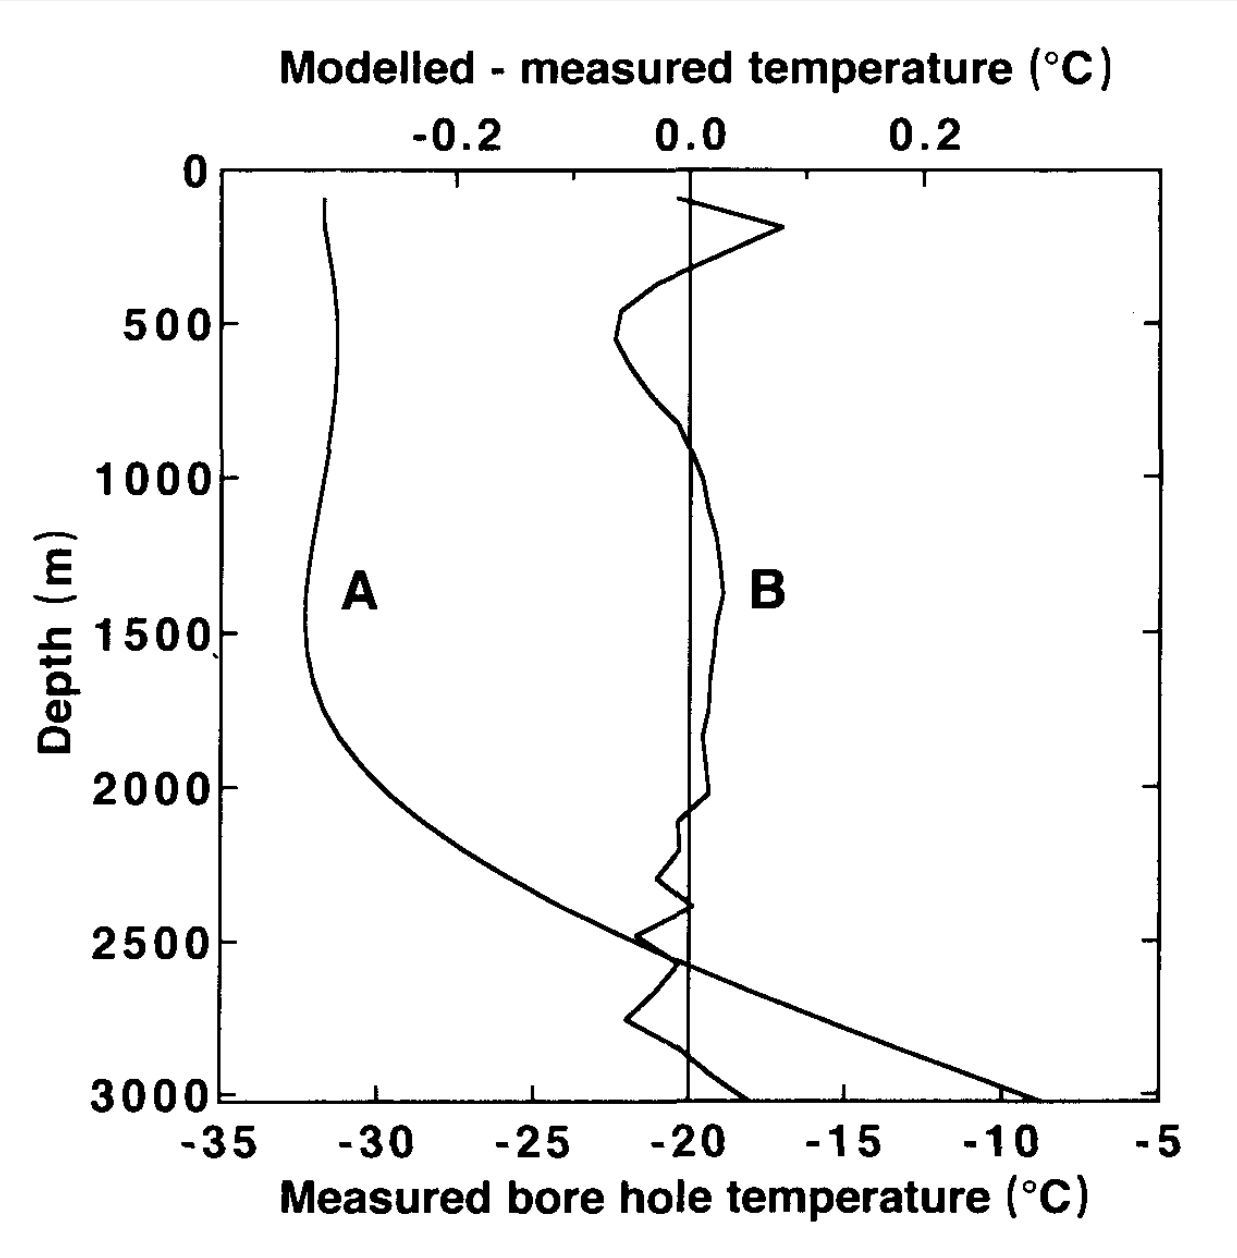
\includegraphics[width=.9\linewidth]{grip/johnsen_1995_fig1.png}
\end{center}

\subsubsection{Thickness}
\label{sec:org64ca639}

\begin{itemize}
\item Reported in \textcite{montagnat_2014} Table 1.
\end{itemize}

\subsubsection{Location}
\label{sec:orgb832537}

\subsubsection{Velocity}
\label{sec:orgb7f5f29}
\clearpage
\subsection{GULL}
\label{sec:org8818506}
\begin{verbatim}
Name                                  | gull
Alternate name                        | GULL
Data source                           | Lüthi, Martin P., Ryser, Claudia, Andrews, Lauren C., Catania, Ginny A., Funk, Martin, Hawley, Robert L., Hoffman, Matthew J., Neumann, Thomas A.: Heat sources within the Greenland Ice Sheet: dissipation, temperate paleo-firn and cryo-hydrologic warming , The Cryosphere 9(1), 245–253, 2015 
Drill year(s)                         | 
Data year(s)                          | 2011-2013
Longitude [°E]                        | -49° 43.093'
Latitude [°N]                         | 69° 27.141'
Approximate location name             | Paakitsoq
Location source                       | Ryser (2014) doi:10.1002/2013JF003067
Ice thickness [m]                     | 700
ice thickness year                    | 
Ice thickness source                  | Ryser (2014) doi:10.1002/2013JF003067
Surface velocity [m yr^-1]            | 
Surface velocity year                 | 
Surface velocity source               | 
Measured from: Top, Bottom, Relative  | T
Depth of top measurement [m]          | 4
Depth of bottom measurement [m]       | 704
\end{verbatim}

\subsubsection{Temperature}
\label{sec:orgde7d063}

\begin{itemize}
\item NOTE: See \href{gull/foxx1/README.org}{FOXX1} for digitization.
\item Digitized from \textcite{luthi_2015} Figure 2:
\end{itemize}

\begin{center}
\includegraphics[width=.9\linewidth]{gull/luthi_2015_fig2_all.png}
\end{center}


\subsubsection{Thickness}
\label{sec:orgb899ffc}

\begin{itemize}
\item From \textcite{ryser_2014_caterpillar}.
\end{itemize}

\subsubsection{Location}
\label{sec:org45f53cd}

\begin{itemize}
\item From \textcite{ryser_2014_caterpillar}.
\end{itemize}

\subsubsection{Velocity}
\label{sec:orgbad3e2c}

\begin{itemize}
\item From \textcite{ryser_2014_caterpillar}.
\end{itemize}

\begin{quote}
Measured surface velocities of about 100 m a−1 are
modulated by seasonal velocity variations; winter
velocities of 70 to 80 m a−1 eventually double during
speedup events in summer. 
\end{quote}
\clearpage
\subsection{H2015\_S1A}
\label{sec:orge5bd596}
\begin{verbatim}
Name                                  | h2015_s1a
Alternate name                        | 
Data source                           | Harrington, Joel A., Humphrey, Neil F., Harper, Joel T.: Temperature distribution and thermal anomalies along a flowline of the Greenland ice sheet , Annals of Glaciology 56(70), 98–104, 2015 
Drill year(s)                         | 
Data year(s)                          | 2011-2013
Longitude [°E]                        | 
Latitude [°N]                         | 
Approximate location name             | 
Location source                       | 
Ice thickness [m]                     | 92
ice thickness year                    | 
Ice thickness source                  | See data source
Surface velocity [m yr^-1]            | 
Surface velocity year                 | 
Surface velocity source               | 
Measured from: Top, Bottom, Relative  | T
Depth of top measurement [m]          | 11.0
Depth of bottom measurement [m]       | 81.0
\end{verbatim}

\subsubsection{Temperature}
\label{sec:org9181cae}

\begin{itemize}
\item From \textcite{harrington_2015} Figure 2
\end{itemize}

\begin{center}
\includegraphics[width=.9\linewidth]{h2015_s1a/harrington_2015_fig2_S1_S2_S3.png}
\end{center}

\subsubsection{Thickness}
\label{sec:org8b3fad0}

\begin{itemize}
\item From \textcite{harrington_2015} Table 1
\end{itemize}

\subsubsection{Location}
\label{sec:org5cbbaa6}

\subsubsection{Velocity}
\label{sec:org427c736}
\clearpage
\subsection{H2015\_S1B}
\label{sec:org125666f}
\begin{verbatim}
Name                                  | h2015_s1b
Alternate name                        | 
Data source                           | Harrington, Joel A., Humphrey, Neil F., Harper, Joel T.: Temperature distribution and thermal anomalies along a flowline of the Greenland ice sheet , Annals of Glaciology 56(70), 98–104, 2015 
Drill year(s)                         | 
Data year(s)                          | 2011-2013
Longitude [°E]                        | 
Latitude [°N]                         | 
Approximate location name             | 
Location source                       | 
Ice thickness [m]                     | 145
ice thickness year                    | 
Ice thickness source                  | See data source
Surface velocity [m yr^-1]            | 
Surface velocity year                 | 
Surface velocity source               | 
Measured from: Top, Bottom, Relative  | T
Depth of top measurement [m]          | 6.0
Depth of bottom measurement [m]       | 131.0
\end{verbatim}

\subsubsection{Temperature}
\label{sec:orga80fbfa}

\begin{itemize}
\item From \textcite{harrington_2015} Figure 2
\item See H2015\_S1A for digitization
\end{itemize}

\begin{center}
\includegraphics[width=.9\linewidth]{h2015_s1b/harrington_2015_fig2_S1_S2_S3.png}
\end{center}

\subsubsection{Thickness}
\label{sec:orgf1c5902}

\begin{itemize}
\item From \textcite{harrington_2015} Table 1
\end{itemize}

\subsubsection{Location}
\label{sec:org90f9df6}

\subsubsection{Velocity}
\label{sec:org4aaa6a8}
\clearpage
\subsection{H2015\_S2A}
\label{sec:orgaff62da}
\begin{verbatim}
Name                                  | h2015_s2a
Alternate name                        | 
Data source                           | Harrington, Joel A., Humphrey, Neil F., Harper, Joel T.: Temperature distribution and thermal anomalies along a flowline of the Greenland ice sheet , Annals of Glaciology 56(70), 98–104, 2015 
Drill year(s)                         | 
Data year(s)                          | 2011-2013
Longitude [°E]                        | 
Latitude [°N]                         | 
Approximate location name             | 
Location source                       | 
Ice thickness [m]                     | 
ice thickness year                    | 
Ice thickness source                  | See data source
Surface velocity [m yr^-1]            | 
Surface velocity year                 | 
Surface velocity source               | 
Measured from: Top, Bottom, Relative  | T
Depth of top measurement [m]          | 3.5
Depth of bottom measurement [m]       | 559
\end{verbatim}

\subsubsection{Temperature}
\label{sec:orgd77c5bd}

\begin{itemize}
\item From \textcite{harrington_2015} Figure 2
\end{itemize}

\begin{center}
\includegraphics[width=.9\linewidth]{h2015_s2a/harrington_2015_fig2_S1_S2_S3.png}
\end{center}

\subsubsection{Thickness}
\label{sec:org580aa8c}

\begin{itemize}
\item Unknown (Use BedMachine after finding location?)
\end{itemize}

\subsubsection{Location}
\label{sec:org25624ce}

\subsubsection{Velocity}
\label{sec:org6140b24}
\clearpage
\subsection{H2015\_S3A}
\label{sec:org5a0ddc4}
\begin{verbatim}
Name                                  | h2015_s3a
Alternate name                        | 
Data source                           | Harrington, Joel A., Humphrey, Neil F., Harper, Joel T.: Temperature distribution and thermal anomalies along a flowline of the Greenland ice sheet , Annals of Glaciology 56(70), 98–104, 2015 
Drill year(s)                         | 
Data year(s)                          | 2011-2013
Longitude [°E]                        | 
Latitude [°N]                         | 
Approximate location name             | 
Location source                       | 
Ice thickness [m]                     | 458
ice thickness year                    | 
Ice thickness source                  | See data source
Surface velocity [m yr^-1]            | 
Surface velocity year                 | 
Surface velocity source               | 
Measured from: Top, Bottom, Relative  | T
Depth of top measurement [m]          | 218.0
Depth of bottom measurement [m]       | 368.0
\end{verbatim}

\subsubsection{Temperature}
\label{sec:org15597f3}

\begin{itemize}
\item From \textcite{harrington_2015} Figure 2
\end{itemize}

\begin{center}
\includegraphics[width=.9\linewidth]{h2015_s3a/harrington_2015_fig2_S1_S2_S3.png}
\end{center}

\subsubsection{Thickness}
\label{sec:org0b3bf4d}

\begin{itemize}
\item From \textcite{harrington_2015} Table 1
\end{itemize}

\subsubsection{Location}
\label{sec:orgc84171b}

\subsubsection{Velocity}
\label{sec:org8f42045}
\clearpage
\subsection{H2015\_S3B}
\label{sec:org91d3ec7}
\begin{verbatim}
Name                                  | h2015_s3b
Alternate name                        | 
Data source                           | Harrington, Joel A., Humphrey, Neil F., Harper, Joel T.: Temperature distribution and thermal anomalies along a flowline of the Greenland ice sheet , Annals of Glaciology 56(70), 98–104, 2015 
Drill year(s)                         | 
Data year(s)                          | 2011-2013
Longitude [°E]                        | 
Latitude [°N]                         | 
Approximate location name             | 
Location source                       | 
Ice thickness [m]                     | 466
ice thickness year                    | 
Ice thickness source                  | See data source
Surface velocity [m yr^-1]            | 
Surface velocity year                 | 
Surface velocity source               | 
Measured from: Top, Bottom, Relative  | T
Depth of top measurement [m]          | 27.0
Depth of bottom measurement [m]       | 460.0
\end{verbatim}

\subsubsection{Temperature}
\label{sec:orgea35fc4}

\begin{itemize}
\item From \textcite{harrington_2015} Figure 2
\item See S3A for digitization file
\end{itemize}

\begin{center}
\includegraphics[width=.9\linewidth]{h2015_s3b/harrington_2015_fig2_S1_S2_S3.png}
\end{center}

\subsubsection{Thickness}
\label{sec:org0395a50}

\begin{itemize}
\item From \textcite{harrington_2015} Table 1
\end{itemize}

\subsubsection{Location}
\label{sec:org8f58c70}

\subsubsection{Velocity}
\label{sec:orge3a4d27}
\clearpage
\subsection{H2015\_S3C}
\label{sec:org9a4fbae}
\begin{verbatim}
Name                                  | h2015_s3c
Alternate name                        | 
Data source                           | Harrington, Joel A., Humphrey, Neil F., Harper, Joel T.: Temperature distribution and thermal anomalies along a flowline of the Greenland ice sheet , Annals of Glaciology 56(70), 98–104, 2015 
Drill year(s)                         | 
Data year(s)                          | 2011-2013
Longitude [°E]                        | 
Latitude [°N]                         | 
Approximate location name             | 
Location source                       | 
Ice thickness [m]                     | 460
ice thickness year                    | 
Ice thickness source                  | See data source
Surface velocity [m yr^-1]            | 
Surface velocity year                 | 
Surface velocity source               | 
Measured from: Top, Bottom, Relative  | T
Depth of top measurement [m]          | 20.0
Depth of bottom measurement [m]       | 459.0
\end{verbatim}

\subsubsection{Temperature}
\label{sec:orgce328d0}

\begin{itemize}
\item From \textcite{harrington_2015} Figure 2
\item See S3A for digitization file
\end{itemize}

\begin{center}
\includegraphics[width=.9\linewidth]{h2015_s3c/harrington_2015_fig2_S1_S2_S3.png}
\end{center}

\subsubsection{Thickness}
\label{sec:org534c304}

\begin{itemize}
\item From \textcite{harrington_2015} Table 1
\end{itemize}

\subsubsection{Location}
\label{sec:orgafc1434}

\subsubsection{Velocity}
\label{sec:org91b8213}
\clearpage
\subsection{H2015\_S4A}
\label{sec:org1dd6c6b}
\begin{verbatim}
Name                                  | h2015_s4a
Alternate name                        | 
Data source                           | Harrington, Joel A., Humphrey, Neil F., Harper, Joel T.: Temperature distribution and thermal anomalies along a flowline of the Greenland ice sheet , Annals of Glaciology 56(70), 98–104, 2015 
Drill year(s)                         | 
Data year(s)                          | 2011-2013
Longitude [°E]                        | 
Latitude [°N]                         | 
Approximate location name             | 
Location source                       | 
Ice thickness [m]                     | 701
Ice thickness year                    | 
Ice thickness source                  | See data source
Surface velocity [m yr^-1]            | 
Surface velocity year                 | 
Surface velocity source               | 
Measured from: Top, Bottom, Relative  | T
Depth of top measurement [m]          | 11.0
Depth of bottom measurement [m]       | 690.0
\end{verbatim}

\subsubsection{Temperature}
\label{sec:orgeff9f97}

\begin{itemize}
\item From \textcite{harrington_2015} Figure 2
\end{itemize}

\begin{center}
\includegraphics[width=.9\linewidth]{h2015_s4a/harrington_2015_fig2_S4_S5.png}
\end{center}

\subsubsection{Thickness}
\label{sec:orgcb8476a}

\begin{itemize}
\item From \textcite{harrington_2015} Table 1
\end{itemize}

\subsubsection{Location}
\label{sec:org02c2ebc}

\subsubsection{Velocity}
\label{sec:org873c46a}
\clearpage
\subsection{H2015\_S4B}
\label{sec:org7d41f43}
\begin{verbatim}
Name                                  | h2015_s4b
Alternate name                        | 
Data source                           | Harrington, Joel A., Humphrey, Neil F., Harper, Joel T.: Temperature distribution and thermal anomalies along a flowline of the Greenland ice sheet , Annals of Glaciology 56(70), 98–104, 2015 
Drill year(s)                         | 
Data year(s)                          | 2011-2013
Longitude [°E]                        | 
Latitude [°N]                         | 
Approximate location name             | 
Location source                       | 
Ice thickness [m]                     | 692
ice thickness year                    | 
Ice thickness source                  | See data source
Surface velocity [m yr^-1]            | 
Surface velocity year                 | 
Surface velocity source               | 
Measured from: Top, Bottom, Relative  | T
Depth of top measurement [m]          | 18.0
Depth of bottom measurement [m]       | 690.0
\end{verbatim}

\subsubsection{Temperature}
\label{sec:orgeecb68d}

\begin{itemize}
\item From \textcite{harrington_2015} Figure 2
\end{itemize}

\begin{center}
\includegraphics[width=.9\linewidth]{h2015_s4b/harrington_2015_fig2_S4_S5.png}
\end{center}

\subsubsection{Thickness}
\label{sec:org83edd08}

\begin{itemize}
\item From \textcite{harrington_2015} Table 1
\end{itemize}

\subsubsection{Location}
\label{sec:org5ad6ab1}

\subsubsection{Velocity}
\label{sec:orgc7b9276}
\clearpage
\subsection{H2015\_S4C}
\label{sec:orgc491906}
\begin{verbatim}
Name                                  | h2015_s4c
Alternate name                        | 
Data source                           | Harrington, Joel A., Humphrey, Neil F., Harper, Joel T.: Temperature distribution and thermal anomalies along a flowline of the Greenland ice sheet , Annals of Glaciology 56(70), 98–104, 2015 
Drill year(s)                         | 
Data year(s)                          | 2011-2013
Longitude [°E]                        | 
Latitude [°N]                         | 
Approximate location name             | 
Location source                       | 
Ice thickness [m]                     | 698
ice thickness year                    | 
Ice thickness source                  | See data source
Surface velocity [m yr^-1]            | 
Surface velocity year                 | 
Surface velocity source               | 
Measured from: Top, Bottom, Relative  | T
Depth of top measurement [m]          | 17.0
Depth of bottom measurement [m]       | 688.0
\end{verbatim}

\subsubsection{Temperature}
\label{sec:org0fcae09}

\begin{itemize}
\item From \textcite{harrington_2015} Figure 2
\end{itemize}

\begin{center}
\includegraphics[width=.9\linewidth]{h2015_s4c/harrington_2015_fig2_S4_S5.png}
\end{center}

\subsubsection{Thickness}
\label{sec:orgb3ffd86}

\begin{itemize}
\item From \textcite{harrington_2015} Table 1
\end{itemize}

\subsubsection{Location}
\label{sec:orgf8a526f}

\subsubsection{Velocity}
\label{sec:org41649d5}
\clearpage
\subsection{H2015\_S5A}
\label{sec:org6566134}
\begin{verbatim}
Name                                  | h2015_s5a
Alternate name                        | 
Data source                           | Harrington, Joel A., Humphrey, Neil F., Harper, Joel T.: Temperature distribution and thermal anomalies along a flowline of the Greenland ice sheet , Annals of Glaciology 56(70), 98–104, 2015 
Drill year(s)                         | 
Data year(s)                          | 2011-2013
Longitude [°E]                        | 
Latitude [°N]                         | 
Approximate location name             | 
Location source                       | 
Ice thickness [m]                     | 821
ice thickness year                    | 
Ice thickness source                  | See data source
Surface velocity [m yr^-1]            | 
Surface velocity year                 | 
Surface velocity source               | 
Measured from: Top, Bottom, Relative  | T
Depth of top measurement [m]          | 1.0
Depth of bottom measurement [m]       | 799.0
\end{verbatim}

\subsubsection{Temperature}
\label{sec:org2827163}

\begin{itemize}
\item From \textcite{harrington_2015} Figure 2
\end{itemize}

\begin{center}
\includegraphics[width=.9\linewidth]{h2015_s5a/harrington_2015_fig2_S4_S5.png}
\end{center}

\subsubsection{Thickness}
\label{sec:orgee39d81}

\begin{itemize}
\item From \textcite{harrington_2015} Table 1
\end{itemize}

\subsubsection{Location}
\label{sec:orgb1199ea}

\subsubsection{Velocity}
\label{sec:org1dab868}
\clearpage
\subsection{H2015\_S5B}
\label{sec:orgdda80e0}
\begin{verbatim}
Name                                  | h2015_s5b
Alternate name                        | 
Data source                           | Harrington, Joel A., Humphrey, Neil F., Harper, Joel T.: Temperature distribution and thermal anomalies along a flowline of the Greenland ice sheet , Annals of Glaciology 56(70), 98–104, 2015 
Drill year(s)                         | 
Data year(s)                          | 2011-2013
Longitude [°E]                        | 
Latitude [°N]                         | 
Approximate location name             | 
Location source                       | 
Ice thickness [m]                     | 815
ice thickness year                    | 
Ice thickness source                  | See data source
Surface velocity [m yr^-1]            | 
Surface velocity year                 | 
Surface velocity source               | 
Measured from: Top, Bottom, Relative  | T
Depth of top measurement [m]          | 114.0
Depth of bottom measurement [m]       | 728.0
\end{verbatim}

\subsubsection{Temperature}
\label{sec:orgfd4beaf}

\begin{itemize}
\item From \textcite{harrington_2015} Figure 2
\end{itemize}

\begin{center}
\includegraphics[width=.9\linewidth]{h2015_s5b/harrington_2015_fig2_S4_S5.png}
\end{center}

\subsubsection{Thickness}
\label{sec:org36efb7f}

\begin{itemize}
\item From \textcite{harrington_2015} Table 1
\end{itemize}

\subsubsection{Location}
\label{sec:org5e09c1e}

\subsubsection{Velocity}
\label{sec:org25fd809}
\clearpage
\subsection{Hans Tausen Dome}
\label{sec:org55070a6}
\begin{verbatim}
Name                                  | hanstausen_dome
Alternate name                        | Hans Tausen Dome
Data source                           | Zekollari, Harry, Huybrechts, Philippe, Noël, Brice, van de Berg, Willem Jan, van den Broeke, Michiel R.: Sensitivity, stability and future evolution of the world’s northernmost ice cap, Hans Tausen Iskappe (Greenland) , The Cryosphere 11(2), Copernicus GmbH, 805–825, 3 2017 
Drill year(s)                         | 
Data year(s)                          | 
Longitude [°E]                        | 
Latitude [°N]                         | 
Approximate location name             | 
Location source                       | 
Ice thickness [m]                     | 345
Ice thickness year                    | 
Ice thickness source                  | See data source
Surface velocity [m yr^-1]            | 
Surface velocity year                 | 
Surface velocity source               | 
Measured from: Top, Bottom, Relative  | B
Depth of top measurement [m]          | 10.0
Depth of bottom measurement [m]       | 344.0
\end{verbatim}

\subsubsection{Temperature}
\label{sec:orgcb48630}

\begin{itemize}
\item From \textcite{zekollari_2017} Figure 6
\end{itemize}
\begin{center}
\includegraphics[width=.9\linewidth]{hanstausen_dome/zekollari_2017_fig6.png}
\end{center}

\subsubsection{Thickness}
\label{sec:orgbb1f25a}

\begin{itemize}
\item From \textcite{zekollari_2017} text.
\end{itemize}

\subsubsection{Location}
\label{sec:org92d0494}

\subsubsection{Velocity}
\label{sec:orgf372721}
\clearpage
\subsection{Hans Tausen Hare}
\label{sec:orga051b5a}
\begin{verbatim}
Name                                  | hanstausen_hare
Alternate name                        | Hans Tausen Hare
Data source                           | Zekollari, Harry, Huybrechts, Philippe, Noël, Brice, van de Berg, Willem Jan, van den Broeke, Michiel R.: Sensitivity, stability and future evolution of the world’s northernmost ice cap, Hans Tausen Iskappe (Greenland) , The Cryosphere 11(2), Copernicus GmbH, 805–825, 3 2017 
Drill year(s)                         | 
Data year(s)                          | 
Longitude [°E]                        | 
Latitude [°N]                         | 
Approximate location name             | 
Location source                       | 
Ice thickness [m]                     | 289
Ice thickness year                    | 
Ice thickness source                  | See data source
Surface velocity [m yr^-1]            | 
Surface velocity year                 | 
Surface velocity source               | 
Measured from: Top, Bottom, Relative  | B
Depth of top measurement [m]          | 10.0
Depth of bottom measurement [m]       | 288.0
\end{verbatim}

\subsubsection{Temperature}
\label{sec:org8bd5c91}

\begin{itemize}
\item From \textcite{zekollari_2017} Figure 6
\item See Hans Tausen Dome folder for digitization file.
\end{itemize}
\begin{center}
\includegraphics[width=.9\linewidth]{hanstausen_hare/zekollari_2017_fig6.png}
\end{center}

\subsubsection{Thickness}
\label{sec:org0908a91}

\begin{itemize}
\item From \textcite{zekollari_2017} text.
\end{itemize}

\subsubsection{Location}
\label{sec:orge95f502}

\subsubsection{Velocity}
\label{sec:orgc366d1e}
\clearpage
\subsection{Isua 10}
\label{sec:orgabd5b42}
\begin{verbatim}
Name                                  | isua_10
Alternate name                        | Isua
Data source                           | Colbeck, S. C., Gow, A. J.: The Margin of the Greenland Ice Sheet at Isua , Journal of Glaciology 24(90), Cambridge University Press (CUP), 155–165, 1979 
Drill year(s)                         | 
Data year(s)                          | 1972-1973
Longitude [°E]                        | -49.75
Latitude [°N]                         | 65.2093
Approximate location name             | 
Location source                       | 
Ice thickness [m]                     | 97
Ice thickness year                    | 
Ice thickness source                  | See data source
Surface velocity [m yr^-1]            | 
Surface velocity year                 | 
Surface velocity source               | 
Measured from: Top, Bottom, Relative  | T
Depth of top measurement [m]          | 5.0
Depth of bottom measurement [m]       | 95.0
\end{verbatim}

\subsubsection{Temperature}
\label{sec:org342c83b}

\begin{itemize}
\item Temperature profiles from \textcite{colbeck_1979} Figure 5.
\end{itemize}

\begin{center}
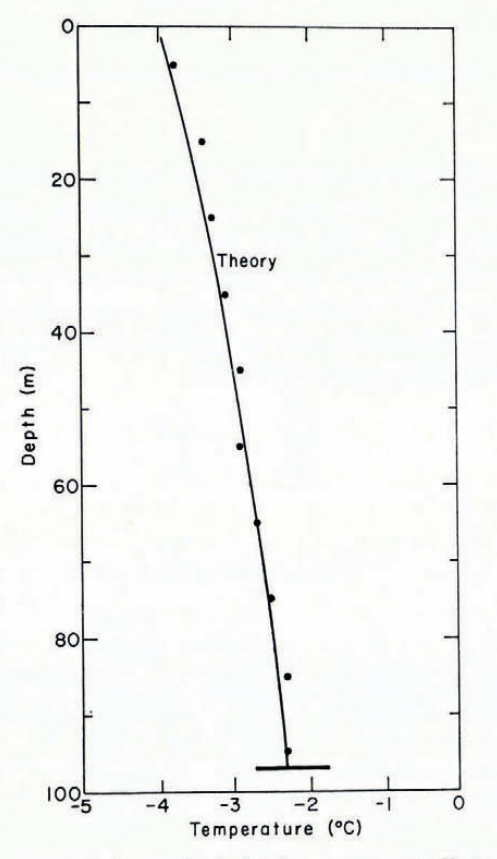
\includegraphics[width=.9\linewidth]{isua_10/isua_10.png}
\end{center}

\subsubsection{Thickness}
\label{sec:org5564125}

\begin{itemize}
\item Thickness from \textcite{colbeck_1979} Table 1.
\end{itemize}

\subsubsection{Location}
\label{sec:org7653cf4}

\begin{itemize}
\item Locations of boreholes from email from WIC: \href{msgid:AM0PR04MB6129F131ECD9123E72752945A2CC0@AM0PR04MB6129.eurprd04.prod.outlook.com}{Isua Site -- SW Greenland}
\end{itemize}

\begin{verbatim}
From: William Colgan
To: Ken Mankoff
Subject: Isua Site -- SW Greenland
Date: Wed 09 Dec 2020 06:58:05 AM PST
Attachments: [1]image002.jpg(147.6K),
 [2]Colbeck1979_fig3_rectif.tfw(122),
 [3]Colbeck1979_fig3_rectif.tif(6.4M),
 [4]Colbeck1979_fig3_rectif.tif.aux.xml(7.9K),
 [5]Colbeck1979_fig3_rectif.tif.ovr(2.1M),
 [6]Colbert1979_core_sites_10-14.cpg(9),
 [7]Colbert1979_core_sites_10-14.dbf(766),
 [8]Colbert1979_core_sites_10-14.prj(568),
 [9]Colbert1979_core_sites_10-14.sbn(256),
 [10]Colbert1979_core_sites_10-14.sbx(171),
 [11]Colbert1979_core_sites_10-14.shp(325),
 [12]Colbert1979_core_sites_10-14.shx(191)
\end{verbatim}

\subsubsection{Velocity}
\label{sec:org6ac5175}
\clearpage
\subsection{Isua 11}
\label{sec:org84301d1}
\begin{verbatim}
Name                                  | isua_11
Alternate name                        | Isua
Data source                           | Colbeck, S. C., Gow, A. J.: The Margin of the Greenland Ice Sheet at Isua , Journal of Glaciology 24(90), Cambridge University Press (CUP), 155–165, 1979 
Drill year(s)                         | 
Data year(s)                          | 1972-1973
Longitude [°E]                        | -49.7510
Latitude [°N]                         | 65.2072
Approximate location name             | 
Location source                       | 
Ice thickness [m]                     | 120
Ice thickness year                    | 
Ice thickness source                  | See data source
Surface velocity [m yr^-1]            | 
Surface velocity year                 | 
Surface velocity source               | 
Measured from: Top, Bottom, Relative  | T
Depth of top measurement [m]          | 25.0
Depth of bottom measurement [m]       | 116.0
\end{verbatim}

\subsubsection{Temperature}
\label{sec:orgaae8da4}

\begin{itemize}
\item Temperature profiles from \textcite{colbeck_1979} Figure 6.
\end{itemize}

\begin{center}
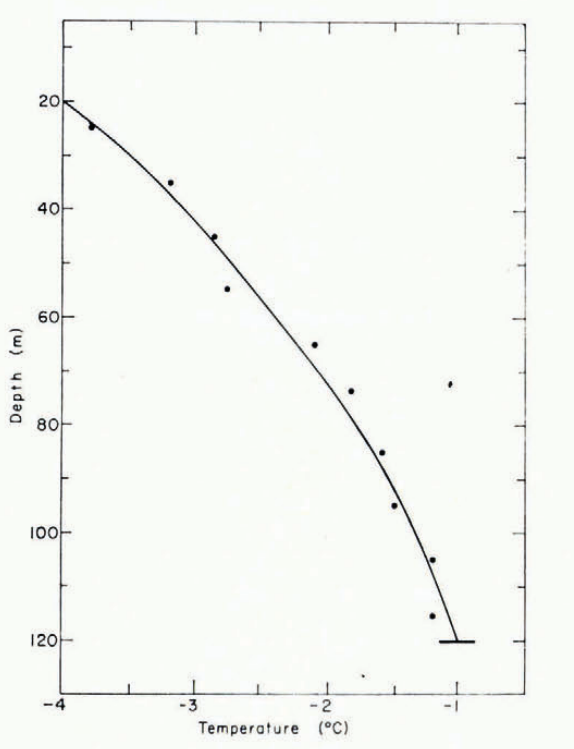
\includegraphics[width=.9\linewidth]{isua_11/isua_11.png}
\end{center}

\subsubsection{Thickness}
\label{sec:orge77507e}

\begin{itemize}
\item Thickness from \textcite{colbeck_1979} Table 1.
\end{itemize}

\subsubsection{Location}
\label{sec:org8ebafbc}

\begin{itemize}
\item Locations of boreholes from email from WIC: \href{msgid:AM0PR04MB6129F131ECD9123E72752945A2CC0@AM0PR04MB6129.eurprd04.prod.outlook.com}{Isua Site -- SW Greenland}
\end{itemize}

\begin{verbatim}
From: William Colgan
To: Ken Mankoff
Subject: Isua Site -- SW Greenland
Date: Wed 09 Dec 2020 06:58:05 AM PST
Attachments: [1]image002.jpg(147.6K),
 [2]Colbeck1979_fig3_rectif.tfw(122),
 [3]Colbeck1979_fig3_rectif.tif(6.4M),
 [4]Colbeck1979_fig3_rectif.tif.aux.xml(7.9K),
 [5]Colbeck1979_fig3_rectif.tif.ovr(2.1M),
 [6]Colbert1979_core_sites_10-14.cpg(9),
 [7]Colbert1979_core_sites_10-14.dbf(766),
 [8]Colbert1979_core_sites_10-14.prj(568),
 [9]Colbert1979_core_sites_10-14.sbn(256),
 [10]Colbert1979_core_sites_10-14.sbx(171),
 [11]Colbert1979_core_sites_10-14.shp(325),
 [12]Colbert1979_core_sites_10-14.shx(191)
\end{verbatim}

\subsubsection{Velocity}
\label{sec:org2de2f8b}
\clearpage
\subsection{Isua 12}
\label{sec:org59dfe5b}
\begin{verbatim}
Name                                  | isua_12
Alternate name                        | Isua
Data source                           | Colbeck, S. C., Gow, A. J.: The Margin of the Greenland Ice Sheet at Isua , Journal of Glaciology 24(90), Cambridge University Press (CUP), 155–165, 1979 
Drill year(s)                         | 
Data year(s)                          | 1972-1973
Longitude [°E]                        | -49.753
Latitude [°N]                         | 65.2039
Approximate location name             | 
Location source                       | 
Ice thickness [m]                     | 100
Ice thickness year                    | 
Ice thickness source                  | See data source
Surface velocity [m yr^-1]            | 
Surface velocity year                 | 
Surface velocity source               | 
Measured from: Top, Bottom, Relative  | T
Depth of top measurement [m]          | 25.0
Depth of bottom measurement [m]       | 95.0
\end{verbatim}

\subsubsection{Temperature}
\label{sec:orgaccc82d}

\begin{itemize}
\item Temperature profiles from \textcite{colbeck_1979} Figure 7.
\end{itemize}

\begin{center}
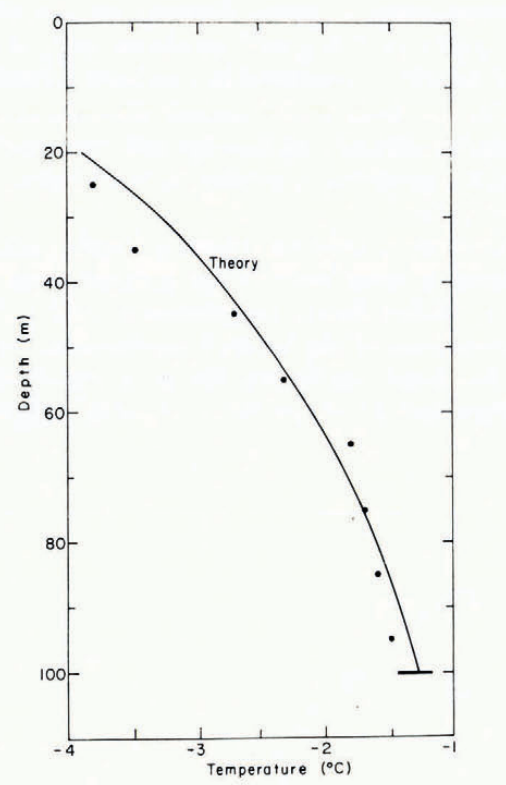
\includegraphics[width=.9\linewidth]{isua_12/isua_12.png}
\end{center}

\subsubsection{Thickness}
\label{sec:orgaacd8f3}

\begin{itemize}
\item Thickness from \textcite{colbeck_1979} Table 1.
\end{itemize}

\subsubsection{Location}
\label{sec:org353e076}

\begin{itemize}
\item Locations of boreholes from email from WIC: \href{msgid:AM0PR04MB6129F131ECD9123E72752945A2CC0@AM0PR04MB6129.eurprd04.prod.outlook.com}{Isua Site -- SW Greenland}
\end{itemize}

\begin{verbatim}
From: William Colgan
To: Ken Mankoff
Subject: Isua Site -- SW Greenland
Date: Wed 09 Dec 2020 06:58:05 AM PST
Attachments: [1]image002.jpg(147.6K),
 [2]Colbeck1979_fig3_rectif.tfw(122),
 [3]Colbeck1979_fig3_rectif.tif(6.4M),
 [4]Colbeck1979_fig3_rectif.tif.aux.xml(7.9K),
 [5]Colbeck1979_fig3_rectif.tif.ovr(2.1M),
 [6]Colbert1979_core_sites_10-14.cpg(9),
 [7]Colbert1979_core_sites_10-14.dbf(766),
 [8]Colbert1979_core_sites_10-14.prj(568),
 [9]Colbert1979_core_sites_10-14.sbn(256),
 [10]Colbert1979_core_sites_10-14.sbx(171),
 [11]Colbert1979_core_sites_10-14.shp(325),
 [12]Colbert1979_core_sites_10-14.shx(191)
\end{verbatim}

\subsubsection{Velocity}
\label{sec:org2ac465a}
\clearpage
\subsection{Isua 13}
\label{sec:orgc561d06}
\begin{verbatim}
Name                                  | isua_13
Alternate name                        | Isua
Data source                           | Colbeck, S. C., Gow, A. J.: The Margin of the Greenland Ice Sheet at Isua , Journal of Glaciology 24(90), Cambridge University Press (CUP), 155–165, 1979 
Drill year(s)                         | 
Data year(s)                          | 1972-1973
Longitude [°E]                        | -49.7456
Latitude [°N]                         | 65.2069
Approximate location name             | 
Location source                       | 
Ice thickness [m]                     | 265
Ice thickness year                    | 
Ice thickness source                  | See data source
Surface velocity [m yr^-1]            | 
Surface velocity year                 | 
Surface velocity source               | 
Measured from: Top, Bottom, Relative  | T
Depth of top measurement [m]          | 6.0
Depth of bottom measurement [m]       | 247.0
\end{verbatim}

\subsubsection{Temperature}
\label{sec:orgb69ae8e}

\begin{itemize}
\item Temperature profiles from \textcite{colbeck_1979} Figure 8.
\end{itemize}

\begin{center}
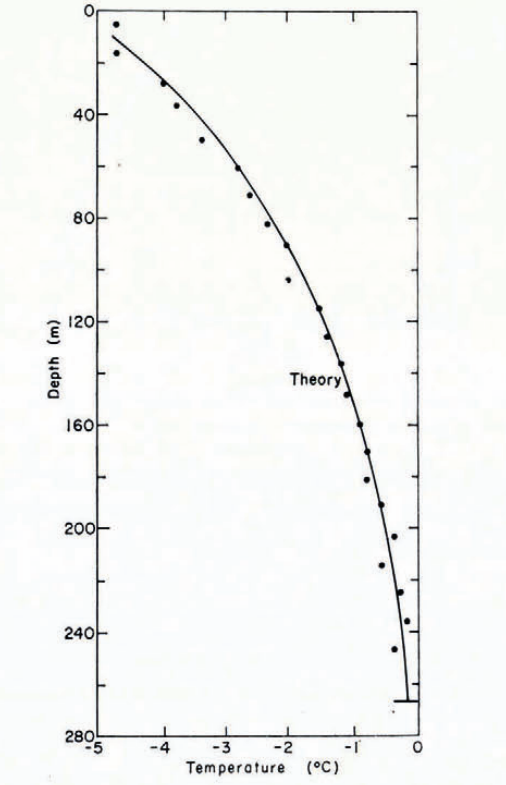
\includegraphics[width=.9\linewidth]{isua_13/isua_13.png}
\end{center}

\subsubsection{Thickness}
\label{sec:org97e0e5e}

\begin{itemize}
\item Thickness from \textcite{colbeck_1979} Table 1.
\end{itemize}

\subsubsection{Location}
\label{sec:org3469543}

\begin{itemize}
\item Locations of boreholes from email from WIC: \href{msgid:AM0PR04MB6129F131ECD9123E72752945A2CC0@AM0PR04MB6129.eurprd04.prod.outlook.com}{Isua Site -- SW Greenland}
\end{itemize}

\begin{verbatim}
From: William Colgan
To: Ken Mankoff
Subject: Isua Site -- SW Greenland
Date: Wed 09 Dec 2020 06:58:05 AM PST
Attachments: [1]image002.jpg(147.6K),
 [2]Colbeck1979_fig3_rectif.tfw(122),
 [3]Colbeck1979_fig3_rectif.tif(6.4M),
 [4]Colbeck1979_fig3_rectif.tif.aux.xml(7.9K),
 [5]Colbeck1979_fig3_rectif.tif.ovr(2.1M),
 [6]Colbert1979_core_sites_10-14.cpg(9),
 [7]Colbert1979_core_sites_10-14.dbf(766),
 [8]Colbert1979_core_sites_10-14.prj(568),
 [9]Colbert1979_core_sites_10-14.sbn(256),
 [10]Colbert1979_core_sites_10-14.sbx(171),
 [11]Colbert1979_core_sites_10-14.shp(325),
 [12]Colbert1979_core_sites_10-14.shx(191)
\end{verbatim}

\subsubsection{Velocity}
\label{sec:org0ed6bba}
\clearpage
\subsection{Isua 14}
\label{sec:org3c4eefc}
\begin{verbatim}
Name                                  | isua_14
Alternate name                        | Isua
Data source                           | Colbeck, S. C., Gow, A. J.: The Margin of the Greenland Ice Sheet at Isua , Journal of Glaciology 24(90), Cambridge University Press (CUP), 155–165, 1979 
Drill year(s)                         | 
Data year(s)                          | 1972-1973
Longitude [°E]                        | -49.7443
Latitude [°N]                         | 65.2058
Approximate location name             | 
Location source                       | 
Ice thickness [m]                     | 299
Ice thickness year                    | 
Ice thickness source                  | See data source
Surface velocity [m yr^-1]            | 
Surface velocity year                 | 
Surface velocity source               | 
Measured from: Top, Bottom, Relative  | T
Depth of top measurement [m]          | 6.0
Depth of bottom measurement [m]       | 237.0
\end{verbatim}

\subsubsection{Temperature}
\label{sec:org3f8db5c}

\begin{itemize}
\item Temperature profiles from \textcite{colbeck_1979} Figure 11.
\end{itemize}

\begin{center}
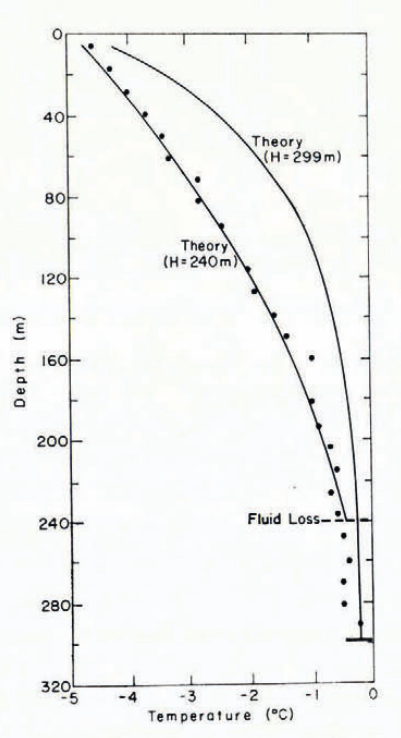
\includegraphics[width=.9\linewidth]{isua_14/isua_14.png}
\end{center}

\subsubsection{Thickness}
\label{sec:org186504e}

\begin{itemize}
\item Thickness from \textcite{colbeck_1979} Table 1.
\end{itemize}

\subsubsection{Location}
\label{sec:orgfea4001}

\begin{itemize}
\item Locations of boreholes from email from WIC: \href{msgid:AM0PR04MB6129F131ECD9123E72752945A2CC0@AM0PR04MB6129.eurprd04.prod.outlook.com}{Isua Site -- SW Greenland}
\end{itemize}

\begin{verbatim}
From: William Colgan
To: Ken Mankoff
Subject: Isua Site -- SW Greenland
Date: Wed 09 Dec 2020 06:58:05 AM PST
Attachments: [1]image002.jpg(147.6K),
 [2]Colbeck1979_fig3_rectif.tfw(122),
 [3]Colbeck1979_fig3_rectif.tif(6.4M),
 [4]Colbeck1979_fig3_rectif.tif.aux.xml(7.9K),
 [5]Colbeck1979_fig3_rectif.tif.ovr(2.1M),
 [6]Colbert1979_core_sites_10-14.cpg(9),
 [7]Colbert1979_core_sites_10-14.dbf(766),
 [8]Colbert1979_core_sites_10-14.prj(568),
 [9]Colbert1979_core_sites_10-14.sbn(256),
 [10]Colbert1979_core_sites_10-14.sbx(171),
 [11]Colbert1979_core_sites_10-14.shp(325),
 [12]Colbert1979_core_sites_10-14.shx(191)
\end{verbatim}

\subsubsection{Velocity}
\label{sec:orgc1610f4}
\clearpage
\subsection{Jakobshavn center}
\label{sec:org1b0df51}
\begin{verbatim}
Name                                  | jakobshavn_center
Alternate name                        | 
Data source                           | Iken, A., Echelmeyer, Κ., Harrison, W., Funk, M.: Mechanisms of fast flow in Jakobshavns Isbræ, West Greenland: Part I. Measurements of temperature and water level in deep boreholes , Journal of Glaciology 39(131), Cambridge University Press (CUP), 15–25, 1993 
Drill year(s)                         | 
Data year(s)                          | 
Longitude [°E]                        | 
Latitude [°N]                         | 
Approximate location name             | 
Location source                       | 
Ice thickness [m]                     | 2495
Ice thickness year                    | 
Ice thickness source                  | See data source
Surface velocity [m yr^-1]            | 
Surface velocity year                 | 
Surface velocity source               | 
Measured from: Top, Bottom, Relative  | T
Depth of top measurement [m]          | 12.0
Depth of bottom measurement [m]       | 2410.0
\end{verbatim}

\subsubsection{Temperature}
\label{sec:orgf028e90}

\begin{itemize}
\item From \textcite{iken_1993} Figure 4 panel b, \(v_p\) digitized
\end{itemize}

\begin{center}
\includegraphics[width=.9\linewidth]{jakobshavn_center/iken_1993_fig4.png}
\end{center}

\subsubsection{Thickness}
\label{sec:org52fc289}

\begin{itemize}
\item From \textcite{iken_1993}.
\end{itemize}

\subsubsection{Location}
\label{sec:orgacd4394}

\subsubsection{Velocity}
\label{sec:org3449df1}
\clearpage
\subsection{Jakobshavn left}
\label{sec:org1c8025c}
\begin{verbatim}
Name                                  | jakobshavn_left
Alternate name                        | 
Data source                           | Iken, A., Echelmeyer, Κ., Harrison, W., Funk, M.: Mechanisms of fast flow in Jakobshavns Isbræ, West Greenland: Part I. Measurements of temperature and water level in deep boreholes , Journal of Glaciology 39(131), Cambridge University Press (CUP), 15–25, 1993 
Drill year(s)                         | 
Data year(s)                          | 
Longitude [°E]                        | 
Latitude [°N]                         | 
Approximate location name             | 
Location source                       | 
Ice thickness [m]                     | 1530
Ice thickness year                    | 
Ice thickness source                  | See data source
Surface velocity [m yr^-1]            | 
Surface velocity year                 | 
Surface velocity source               | 
Measured from: Top, Bottom, Relative  | T
Depth of top measurement [m]          | 8.0
Depth of bottom measurement [m]       | 1517.0
\end{verbatim}

\subsubsection{Temperature}
\label{sec:org1ab5e19}

\begin{itemize}
\item From \textcite{iken_1993} Figure 4 panel b, \(v_p\) digitized
\end{itemize}
\begin{center}
\includegraphics[width=.9\linewidth]{jakobshavn_left/iken_1993_fig4.png}
\end{center}

\subsubsection{Thickness}
\label{sec:org1eb2aed}

\begin{itemize}
\item From \textcite{iken_1993}.
\end{itemize}

\subsubsection{Location}
\label{sec:orgf907be9}

\subsubsection{Velocity}
\label{sec:org3a1fe63}
\clearpage
\subsection{Jakobshavn sheet}
\label{sec:org119c10b}
\begin{verbatim}
Name                                  | jakobshavn_sheet
Alternate name                        | 
Data source                           | Lüthi, Martin, Funk, Martin, Iken, Almut, Gogineni, Shivaprasad, Truffer, Martin: Mechanisms of fast flow in Jakobshavns Isbræ, West Greenland: Part III. Measurements of ice deformation, temperature and cross-borehole conductivity in boreholes to the bedrock , Journal of Glaciology 48(162), 369–385, 2002 
Drill year(s)                         | 
Data year(s)                          | 
Longitude [°E]                        | 
Latitude [°N]                         | 
Approximate location name             | 
Location source                       | 
Ice thickness [m]                     | 828
Ice thickness year                    | 
Ice thickness source                  | See data source
Surface velocity [m yr^-1]            | 
Surface velocity year                 | 
Surface velocity source               | 
Measured from: Top, Bottom, Relative  | T
Depth of top measurement [m]          | 19.0
Depth of bottom measurement [m]       | 798.0
\end{verbatim}

\subsubsection{Temperature}
\label{sec:org2a64729}

\begin{itemize}
\item From \textcite{luthi_2002} Figure 7 (a)
\item Additional profiles (margin, centre) are from \textcite{iken_1993} and named "jakobshavn\_center" and "jakobshavn\_left".
\end{itemize}
\begin{center}
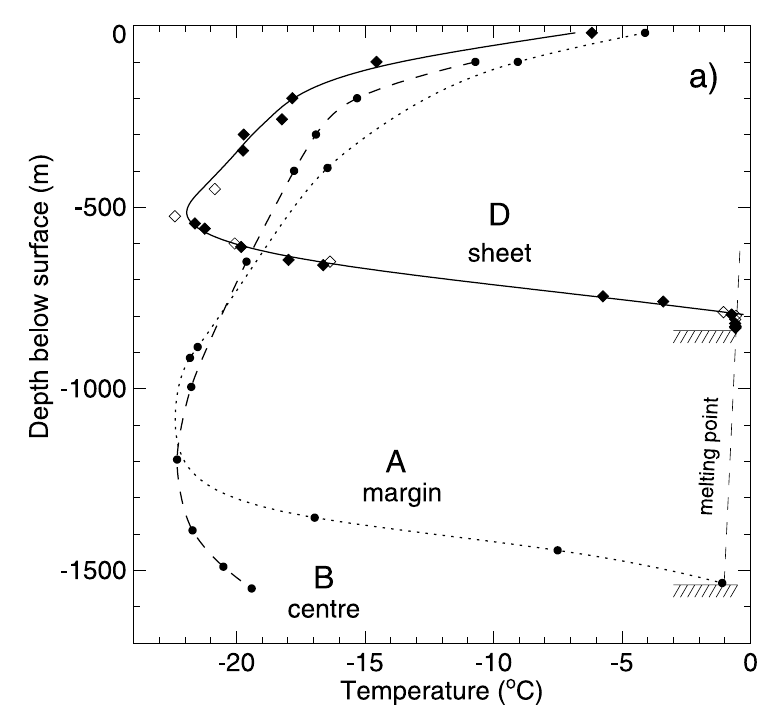
\includegraphics[width=.9\linewidth]{jakobshavn_sheet/luthi_2002_fig7.png}
\end{center}


\subsubsection{Thickness}
\label{sec:org3a9e99a}

\begin{itemize}
\item From \textcite{luthi_2002}.
\end{itemize}

\subsubsection{Location}
\label{sec:org9629856}

\subsubsection{Velocity}
\label{sec:orgdcb9bb0}
\clearpage
\subsection{McDowell (2020) 14N}
\label{sec:org7f1b321}
\begin{verbatim}
Name                                  | mcdowell_2021_14n
Alternate name                        | 
Data source                           |  McDowell, I. E., Humphrey, N. F., Harper, J. T., and Meierbachtol, T. W.: The cooling signature of basal crevasses in a hard-bedded region of the Greenland Ice Sheet, The Cryosphere, 15, 897–907, https://doi.org/10.5194/tc-15-897-2021, 2021.
Drill year(s)                         | 2014
Data year(s)                          | August 2015
Longitude [°E]                        | -49.57231502
Latitude [°N]                         | 67.18300296
Approximate location name             | 
Location source                       | 
Ice thickness [m]                     | 641
Ice thickness year                    | 2014
Ice thickness source                  | See raw data file `Greenland_AblationZone_TProfiles.xlsx` in 14n folder
Surface velocity [m yr^-1]            | 
Surface velocity year                 | 
Surface velocity source               | 
Measured from: Top, Bottom, Relative  | B
Depth of top measurement [m]          | 18
Depth of bottom measurement [m]       | 623
\end{verbatim}

\subsubsection{Temperature}
\label{sec:orgf58b814}

\begin{itemize}
\item Provided by Ian McDowell (see raw data file `Greenland\_AblationZone\_TProfiles.xlsx` in 14n folder)
\end{itemize}

\subsubsection{Thickness}
\label{sec:orgc8af5e4}

\begin{itemize}
\item Provided by Ian McDowell (see raw data file `Greenland\_AblationZone\_TProfiles.xlsx` in 14n folder)
\end{itemize}

\subsubsection{Location}
\label{sec:org5a70213}

\begin{itemize}
\item Provided by Ian McDowell (see raw data file `Greenland\_AblationZone\_TProfiles.xlsx` in 14n folder)
\end{itemize}

\subsubsection{Velocity}
\label{sec:org651079d}
\clearpage
\subsection{McDowell (2020) 14SA}
\label{sec:org500c300}
\begin{verbatim}
Name                                  | mcdowell_2021_14sa
Alternate name                        | 
Data source                           |  McDowell, I. E., Humphrey, N. F., Harper, J. T., and Meierbachtol, T. W.: The cooling signature of basal crevasses in a hard-bedded region of the Greenland Ice Sheet, The Cryosphere, 15, 897–907, https://doi.org/10.5194/tc-15-897-2021, 2021.
Drill year(s)                         | 2014
Data year(s)                          | August 2015
Longitude [°E]                        | -49.57241703
Latitude [°N]                         | 67.180997
Approximate location name             | 
Location source                       | 
Ice thickness [m]                     | 674
Ice thickness year                    | 2014
Ice thickness source                  | See raw data file `Greenland_AblationZone_TProfiles.xlsx` in 14n folder
Surface velocity [m yr^-1]            | 
Surface velocity year                 | 
Surface velocity source               | 
Measured from: Top, Bottom, Relative  | B
Depth of top measurement [m]          | 72
Depth of bottom measurement [m]       | 672
\end{verbatim}

\subsubsection{Temperature}
\label{sec:org6b4b784}

\begin{itemize}
\item Provided by Ian McDowell (see raw data file `Greenland\_AblationZone\_TProfiles.xlsx` in 14n folder)
\end{itemize}

\subsubsection{Thickness}
\label{sec:org78777b8}

\begin{itemize}
\item Provided by Ian McDowell (see raw data file `Greenland\_AblationZone\_TProfiles.xlsx` in 14n folder)
\end{itemize}

\subsubsection{Location}
\label{sec:org8b51f47}

\begin{itemize}
\item Provided by Ian McDowell (see raw data file `Greenland\_AblationZone\_TProfiles.xlsx` in 14n folder)
\end{itemize}

\subsubsection{Velocity}
\label{sec:org63b3212}
\clearpage
\subsection{McDowell (2020) 14SB}
\label{sec:org909041d}
\begin{verbatim}
Name                                  | mcdowell_2021_14sb
Alternate name                        | 
Data source                           |  McDowell, I. E., Humphrey, N. F., Harper, J. T., and Meierbachtol, T. W.: The cooling signature of basal crevasses in a hard-bedded region of the Greenland Ice Sheet, The Cryosphere, 15, 897–907, https://doi.org/10.5194/tc-15-897-2021, 2021.
Drill year(s)                         | 2014
Data year(s)                          | August 2015
Longitude [°E]                        | -49.57216096
Latitude [°N]                         | 67.18095903
Approximate location name             | 
Location source                       | 
Ice thickness [m]                     | 677
Ice thickness year                    | 2014
Ice thickness source                  | See raw data file `Greenland_AblationZone_TProfiles.xlsx` in 14n folder
Surface velocity [m yr^-1]            | 
Surface velocity year                 | 
Surface velocity source               | 
Measured from: Top, Bottom, Relative  | B
Depth of top measurement [m]          | 496
Depth of bottom measurement [m]       | 676
\end{verbatim}

\subsubsection{Temperature}
\label{sec:org2463e39}

\begin{itemize}
\item Provided by Ian McDowell (see raw data file `Greenland\_AblationZone\_TProfiles.xlsx` in 14n folder)
\end{itemize}

\subsubsection{Thickness}
\label{sec:org7326f13}

\begin{itemize}
\item Provided by Ian McDowell (see raw data file `Greenland\_AblationZone\_TProfiles.xlsx` in 14n folder)
\end{itemize}

\subsubsection{Location}
\label{sec:org1420909}

\begin{itemize}
\item Provided by Ian McDowell (see raw data file `Greenland\_AblationZone\_TProfiles.xlsx` in 14n folder)
\end{itemize}

\subsubsection{Velocity}
\label{sec:orgac9db64}
\clearpage
\subsection{McDowell (2020) 14W}
\label{sec:orgfe651fa}
\begin{verbatim}
Name                                  | mcdowell_2021_14w
Alternate name                        | 
Data source                           |  McDowell, I. E., Humphrey, N. F., Harper, J. T., and Meierbachtol, T. W.: The cooling signature of basal crevasses in a hard-bedded region of the Greenland Ice Sheet, The Cryosphere, 15, 897–907, https://doi.org/10.5194/tc-15-897-2021, 2021.
Drill year(s)                         | 2014
Data year(s)                          | August 2015
Longitude [°E]                        | -49.57478802
Latitude [°N]                         | 67.18201398
Approximate location name             | 
Location source                       | 
Ice thickness [m]                     | 661
Ice thickness year                    | 2014
Ice thickness source                  | See raw data file `Greenland_AblationZone_TProfiles.xlsx` in 14n folder
Surface velocity [m yr^-1]            | 
Surface velocity year                 | 
Surface velocity source               | 
Measured from: Top, Bottom, Relative  | B
Depth of top measurement [m]          | 40
Depth of bottom measurement [m]       | 660
\end{verbatim}

\subsubsection{Temperature}
\label{sec:orgc1b2052}

\begin{itemize}
\item Provided by Ian McDowell (see raw data file `Greenland\_AblationZone\_TProfiles.xlsx` in 14n folder)
\end{itemize}

\subsubsection{Thickness}
\label{sec:org7ecd6d6}

\begin{itemize}
\item Provided by Ian McDowell (see raw data file `Greenland\_AblationZone\_TProfiles.xlsx` in 14n folder)
\end{itemize}

\subsubsection{Location}
\label{sec:orgfccbb9a}

\begin{itemize}
\item Provided by Ian McDowell (see raw data file `Greenland\_AblationZone\_TProfiles.xlsx` in 14n folder)
\end{itemize}

\subsubsection{Velocity}
\label{sec:orgb4088b4}
\clearpage
\subsection{McDowell (2020) 14CA}
\label{sec:orgb8ebcc7}
\begin{verbatim}
Name                                  | mcdowell_2021_15ca
Alternate name                        | 
Data source                           |  McDowell, I. E., Humphrey, N. F., Harper, J. T., and Meierbachtol, T. W.: The cooling signature of basal crevasses in a hard-bedded region of the Greenland Ice Sheet, The Cryosphere, 15, 897–907, https://doi.org/10.5194/tc-15-897-2021, 2021.
Drill year(s)                         | 2015
Data year(s)                          | August 2016
Longitude [°E]                        | -49.56950398
Latitude [°N]                         | 67.182104
Approximate location name             | 
Location source                       | 
Ice thickness [m]                     | 671
Ice thickness year                    | 2015
Ice thickness source                  | See raw data file `Greenland_AblationZone_TProfiles.xlsx` in 14n folder
Surface velocity [m yr^-1]            | 
Surface velocity year                 | 
Surface velocity source               | 
Measured from: Top, Bottom, Relative  | B
Depth of top measurement [m]          | 46
Depth of bottom measurement [m]       | 666
\end{verbatim}

\subsubsection{Temperature}
\label{sec:org9ab2ab6}

\begin{itemize}
\item Provided by Ian McDowell (see raw data file `Greenland\_AblationZone\_TProfiles.xlsx` in 14n folder)
\end{itemize}

\subsubsection{Thickness}
\label{sec:orgc4900fa}

\begin{itemize}
\item Provided by Ian McDowell (see raw data file `Greenland\_AblationZone\_TProfiles.xlsx` in 14n folder)
\end{itemize}

\subsubsection{Location}
\label{sec:orgf3ecb2e}

\begin{itemize}
\item Provided by Ian McDowell (see raw data file `Greenland\_AblationZone\_TProfiles.xlsx` in 14n folder)
\end{itemize}

\subsubsection{Velocity}
\label{sec:org2ff19ad}
\clearpage
\subsection{McDowell (2020) 14CB}
\label{sec:orge677acb}
\begin{verbatim}
Name                                  | mcdowell_2021_15cb
Alternate name                        | 
Data source                           |  McDowell, I. E., Humphrey, N. F., Harper, J. T., and Meierbachtol, T. W.: The cooling signature of basal crevasses in a hard-bedded region of the Greenland Ice Sheet, The Cryosphere, 15, 897–907, https://doi.org/10.5194/tc-15-897-2021, 2021.
Drill year(s)                         | 2015
Data year(s)                          | August 2016
Longitude [°E]                        | -49.569493
Latitude [°N]                         | 67.18201297
Approximate location name             | 
Location source                       | 
Ice thickness [m]                     | 675
Ice thickness year                    | 2015
Ice thickness source                  | See raw data file `Greenland_AblationZone_TProfiles.xlsx` in 14n folder
Surface velocity [m yr^-1]            | 
Surface velocity year                 | 
Surface velocity source               | 
Measured from: Top, Bottom, Relative  | B
Depth of top measurement [m]          | 370
Depth of bottom measurement [m]       | 670
\end{verbatim}

\subsubsection{Temperature}
\label{sec:orgfc86ff4}

\begin{itemize}
\item Provided by Ian McDowell (see raw data file `Greenland\_AblationZone\_TProfiles.xlsx` in 14n folder)
\end{itemize}

\subsubsection{Thickness}
\label{sec:orgaedcd8e}

\begin{itemize}
\item Provided by Ian McDowell (see raw data file `Greenland\_AblationZone\_TProfiles.xlsx` in 14n folder)
\end{itemize}

\subsubsection{Location}
\label{sec:org0b0286c}

\begin{itemize}
\item Provided by Ian McDowell (see raw data file `Greenland\_AblationZone\_TProfiles.xlsx` in 14n folder)
\end{itemize}

\subsubsection{Velocity}
\label{sec:org786ab1c}
\clearpage
\subsection{McDowell (2020) 15E}
\label{sec:orgb3621d2}
\begin{verbatim}
Name                                  | mcdowell_2021_15e
Alternate name                        | 
Data source                           |  McDowell, I. E., Humphrey, N. F., Harper, J. T., and Meierbachtol, T. W.: The cooling signature of basal crevasses in a hard-bedded region of the Greenland Ice Sheet, The Cryosphere, 15, 897–907, https://doi.org/10.5194/tc-15-897-2021, 2021.
Drill year(s)                         | 2015
Data year(s)                          | August 2016
Longitude [°E]                        | -49.56402498
Latitude [°N]                         | 67.18186604
Approximate location name             | 
Location source                       | 
Ice thickness [m]                     | 665
Ice thickness year                    | 2015
Ice thickness source                  | See raw data file `Greenland_AblationZone_TProfiles.xlsx` in 14n folder
Surface velocity [m yr^-1]            | 
Surface velocity year                 | 
Surface velocity source               | 
Measured from: Top, Bottom, Relative  | B
Depth of top measurement [m]          | 40
Depth of bottom measurement [m]       | 660
\end{verbatim}

\subsubsection{Temperature}
\label{sec:org26b1d29}

\begin{itemize}
\item Provided by Ian McDowell (see raw data file `Greenland\_AblationZone\_TProfiles.xlsx` in 14n folder)
\end{itemize}

\subsubsection{Thickness}
\label{sec:orgbb41df2}

\begin{itemize}
\item Provided by Ian McDowell (see raw data file `Greenland\_AblationZone\_TProfiles.xlsx` in 14n folder)
\end{itemize}

\subsubsection{Location}
\label{sec:orgdba2f02}

\begin{itemize}
\item Provided by Ian McDowell (see raw data file `Greenland\_AblationZone\_TProfiles.xlsx` in 14n folder)
\end{itemize}

\subsubsection{Velocity}
\label{sec:org293848e}
\clearpage
\subsection{McDowell (2020) 15n}
\label{sec:orge9ac972}
\begin{verbatim}
Name                                  | mcdowell_2021_15n
Alternate name                        | 
Data source                           |  McDowell, I. E., Humphrey, N. F., Harper, J. T., and Meierbachtol, T. W.: The cooling signature of basal crevasses in a hard-bedded region of the Greenland Ice Sheet, The Cryosphere, 15, 897–907, https://doi.org/10.5194/tc-15-897-2021, 2021.
Drill year(s)                         | 2015
Data year(s)                          | August 2016
Longitude [°E]                        | -49.56691397
Latitude [°N]                         | 67.183124
Approximate location name             | 
Location source                       | 
Ice thickness [m]                     | 640
Ice thickness year                    | 2015
Ice thickness source                  | See raw data file `Greenland_AblationZone_TProfiles.xlsx` in 14n folder
Surface velocity [m yr^-1]            | 
Surface velocity year                 | 
Surface velocity source               | 
Measured from: Top, Bottom, Relative  | B
Depth of top measurement [m]          | 15
Depth of bottom measurement [m]       | 635
\end{verbatim}

\subsubsection{Temperature}
\label{sec:orgfaa830a}

\begin{itemize}
\item Provided by Ian McDowell (see raw data file `Greenland\_AblationZone\_TProfiles.xlsx` in 14n folder)
\end{itemize}

\subsubsection{Thickness}
\label{sec:org6db9386}

\begin{itemize}
\item Provided by Ian McDowell (see raw data file `Greenland\_AblationZone\_TProfiles.xlsx` in 14n folder)
\end{itemize}

\subsubsection{Location}
\label{sec:orgff900fd}

\begin{itemize}
\item Provided by Ian McDowell (see raw data file `Greenland\_AblationZone\_TProfiles.xlsx` in 14n folder)
\end{itemize}

\subsubsection{Velocity}
\label{sec:org8ebad74}
\clearpage
\subsection{McDowell (2020) 15s}
\label{sec:org95701ce}
\begin{verbatim}
Name                                  | mcdowell_2021_15s
Alternate name                        | 
Data source                           |  McDowell, I. E., Humphrey, N. F., Harper, J. T., and Meierbachtol, T. W.: The cooling signature of basal crevasses in a hard-bedded region of the Greenland Ice Sheet, The Cryosphere, 15, 897–907, https://doi.org/10.5194/tc-15-897-2021, 2021.
Drill year(s)                         | 2015
Data year(s)                          | August 2016
Longitude [°E]                        | -49.56666302
Latitude [°N]                         | 67.180939
Approximate location name             | 
Location source                       | 
Ice thickness [m]                     | 677
Ice thickness year                    | 2015
Ice thickness source                  | See raw data file `Greenland_AblationZone_TProfiles.xlsx` in 14n folder
Surface velocity [m yr^-1]            | 
Surface velocity year                 | 
Surface velocity source               | 
Measured from: Top, Bottom, Relative  | B
Depth of top measurement [m]          | 52
Depth of bottom measurement [m]       | 672
\end{verbatim}

\subsubsection{Temperature}
\label{sec:orge53f0a1}

\begin{itemize}
\item Provided by Ian McDowell (see raw data file `Greenland\_AblationZone\_TProfiles.xlsx` in 14n folder)
\end{itemize}

\subsubsection{Thickness}
\label{sec:org0248b8f}

\begin{itemize}
\item Provided by Ian McDowell (see raw data file `Greenland\_AblationZone\_TProfiles.xlsx` in 14n folder)
\end{itemize}

\subsubsection{Location}
\label{sec:org1cb9c2f}

\begin{itemize}
\item Provided by Ian McDowell (see raw data file `Greenland\_AblationZone\_TProfiles.xlsx` in 14n folder)
\end{itemize}

\subsubsection{Velocity}
\label{sec:org6fc60a1}
\clearpage
\subsection{Meighen}
\label{sec:org93aec96}
\begin{verbatim}
Name                                  | meighen
Alternate name                        | Meighen Ice Cap
Data source                           | Paterson, W. S. B.: A temperature profile through the Meighen ice cap, Arctic Canada , International Association of Scientific Hydrology 79, 440–449, 1968 
Drill year(s)                         | 
Data year(s)                          | 1965
Longitude [°E]                        | 
Latitude [°N]                         | 
Approximate location name             | 
Location source                       | 
Ice thickness [m]                     | 121.2
Ice thickness year                    | 
Ice thickness source                  | See data source
Surface velocity [m yr^-1]            | 
Surface velocity year                 | 
Surface velocity source               | 
Measured from: Top, Bottom, Relative  | T
Depth of top measurement [m]          | 1.0
Depth of bottom measurement [m]       | 121.0
\end{verbatim}

\subsubsection{Temperature}
\label{sec:orgbc756b5}

\begin{itemize}
\item Table (no graphic) from \textcite{paterson_1968} Table 1.
\item Result is average of 1966 and 1967 columns.
\end{itemize}

\subsubsection{Thickness}
\label{sec:org766730b}

\begin{itemize}
\item From \textcite{paterson_1968}.
\end{itemize}

\subsubsection{Location}
\label{sec:org21ae4f3}

\subsubsection{Velocity}
\label{sec:org2295934}
\clearpage
\subsection{NEEM}
\label{sec:org1f76406}
\begin{verbatim}
Name                                  | neem
Alternate name                        | NEEM
Data source                           | MacGregor, Joseph A., Li, Jilu, Paden, John D., Catania, Ginny A., Clow, Gary D., Fahnestock, Mark A., Gogineni, S. Prasad, Grimm, Robert E., Morlighem, Mathieu, Nandi, Soumyaroop, et al.: Radar attenuation and temperature within the Greenland Ice Sheet , Journal of Geophysical Research: Earth Surface 120(6), American Geophysical Union (AGU), 983–1008, 6 2015 
Drill year(s)                         | 2008 through 2012
Data year(s)                          | 2011
Longitude [°E]                        | -51.06
Latitude [°N]                         | 77.45
Approximate location name             | Northwest Greenland
Location source                       | Dahl-Jensen, D., Albert, Mary R., Aldahan, A., Azuma, N., Balslev-Clausen, D., Baumgartner, M., Berggren, A. -M., Bigler, M., Binder, T., Blunier, T., Bourgeois, J. C., Brook, E. J., Buchardt, S. L., Buizert, C., Capron, E., Chappellaz, J., Chung, J., Clausen, H. B., Cvijanovic, I., Davies, S. M., Ditlevsen, P., Eicher, O., Fischer, H., Fisher, D. A., Fleet, L. G., Gfeller, G., Gkinis, V., Gogineni, S., Goto-Azuma, K., Grinsted, A., Gudlaugsdottir, H., Guillevic, M., Hansen, S. B., Hansson, M., Hirabayashi, M., Hong, S., Hur, S. D., Huybrechts, Philippe, Hvidberg, C. S., Iizuka, Y., Jenk, T., Johnsen, S. J., Jones, T. R., Jouzel, J., Karlsson, N. B., Kawamura, K., Keegan, K., Kettner, E., Kipfstuhl, S., Kjær, H. A., Koutnik, M., Kuramoto, T., Koehler, P., Laepple, T., Landais, A., Langen, P. L., Larsen, L. B., Leuenberger, D., Leuenberger, M., Leuschen, C., Li, J., Lipenkov, V., Martinerie, P., Maselli, O. J., Masson-Delmotte, V., McConnell, J. R., Miller, H., Mini, O., Miyamoto, A., Montagnat-Rentier, M., Mulvaney, R., Muscheler, Raimund, Orsi, A. J., Paden, J., Panton, C., Pattyn, F., Petit, J. -R., Pol, K., Popp, T., Possnert, G., Prie, F., Prokopiou, M., Quiquet, A., Rasmussen, S. O., Raynaud, D., Ren, J., Reutenauer, C., Ritz, C., Rockmann, T., Rosen, J. L., Rubino, M., Rybak, O., Samyn, D., Sapart, C. J., Schilt, A., Schmidt, A. M. Z., Schwander, J., Schuepbach, S., Seierstad, I., Severinghaus, J. P., Sheldon, S., Simonsen, S. B., Sjolte, Jesper, Solgaard, A. M., Sowers, T., Sperlich, P., Steen-Larsen, H. C., Steffen, K., Steffensen, J. P., Steinhage, D., Stocker, T. F., Stowasser, C., Sturevik, A. S., Sturges, W. T., Sveinbjornsdottir, A., Svensson, A., Tison, J. -L., Uetake, J., Vallelonga, P., van de Wal, R. S. W., van der Wel, G., Vaughn, B. H., Vinther, B., Waddington, E., Wegner, A., Weikusat, I., White, J. W. C., Wilhelms, F., Winstrup, M., Witrant, E., Wolff, E. W., Xiao, C., Zheng, J.: Eemian interglacial reconstructed from a Greenland folded ice core , Nature 493(7433), Nature Publishing Group, 489–494, 2013 
Ice thickness [m]                     | 2538
Ice thickness year                    | 
Ice thickness source                  | MacGregor, Joseph A., Fahnestock, Mark A., Catania, Ginny A., Aschwanden, Andy, Clow, Gary D., Colgan, William T., Gogineni, Prasad S., Morlighem, Mathieu, Nowicki, Sophie M. J., Paden, John D., Price, Stephen F., Seroussi, Hélène: A synthesis of the basal thermal state of the Greenland Ice Sheet , Journal of Geophysical Research: Earth Surface 121(7), 1328–1350, 2016 
Surface velocity [m yr^-1]            | 
Surface velocity year                 | 
Surface velocity source               | 
Measured from: Top, Bottom, Relative  | R
Depth of top measurement [m]          | 91.0
Depth of bottom measurement [m]       | 2509.0
\end{verbatim}

\subsubsection{Temperature}
\label{sec:org4a51c2a}

\begin{itemize}
\item Data provided by 3rd party in MAT format, converted to CSV
\begin{itemize}
\item Email 1: \href{msgid:C1563C1B-084B-428B-9799-26BE88858CD7@nasa.gov}{Re: [EXTERNAL] Re: GISP2 temperature profile}
\item Email 2: \href{msgid:CACoJM5tpXAdV=eayGpZpJ\_oydjTAxc064rNmXHFE5zDKEq\_yYA@mail.gmail.com}{Fwd: NEEM temperature profile}
\end{itemize}
\item See also \textcite{macgregor_2015} Figure 6.
\end{itemize}

\begin{verbatim}
From: MacGregor, Joseph (GSFC-6150)
To: Ken Mankoff
Subject: Re: [EXTERNAL] Re: GISP2 temperature profile
Date: Wed 06 Jan 2021 03:27:40 PM PST
Attachments: [1]neem_temp.mat(5.0K), [2]NEEM_Tz.pdf(99.3K),
 [3]NEEM-D_11MAY30b_50m.txt(1.9K)

See attached for NEEM [...] includes a mild linear interpolation to handle the convection cells because it was year 1 for that measurement. The original data and a plot from Gary [Clow] also attached. [...] he presumably re-measured in 2015, so it may be technically true that the "final" NEEM temperature profile is not published.
\end{verbatim}

\subsubsection{Thickness}
\label{sec:org8ea7704}

\begin{itemize}
\item Reported as 2540 in \textcite{dahl-jensen_2013}.
\item Reported as 2538 in \textcite{macgregor_2016}, with some extra details in Table 1.
\end{itemize}

\subsubsection{Location}
\label{sec:org8a03200}

\begin{itemize}
\item From \textcite{dahl-jensen_2013}.
\end{itemize}

\subsubsection{Velocity}
\label{sec:org6342e17}
\clearpage
\subsection{NGRIP}
\label{sec:org180f421}
\begin{verbatim}
Name                                  | ngrip
Alternate name                        | NGRIP
Data source                           | Dahl-Jensen, Dorthe, Gundestrup, Niels, Gogineni, S Prasad, Miller, Heinz: Basal melt at NorthGRIP modeled from borehole, ice-core and radio-echo sounder observations , Annals of Glaciology 37, International Glaciological Society, 207–212, 2003 
Drill year(s)                         | 1996-2004 (Vinther, 2008)
Data year(s)                          | 
Longitude [°E]                        | -42.32
Latitude [°N]                         | 75.10
Approximate location name             | 
Location source                       | Vinther (2008)
Ice thickness [m]                     | 3080
Ice thickness year                    | 
Ice thickness source                  | See data source
Surface velocity [m yr^-1]            | 
Surface velocity year                 | 
Surface velocity source               | 
Measured from: Top, Bottom, Relative  | T
Depth of top measurement [m]          | 204.0
Depth of bottom measurement [m]       | 2888.0
\end{verbatim}

\subsubsection{Temperature}
\label{sec:org5b52428}

\begin{itemize}
\item From \textcite{dahl-jensen_2003} Figure 1. Black line digitized as NGRIP. Gray line is GRIP temperature profile.
\end{itemize}
\begin{center}
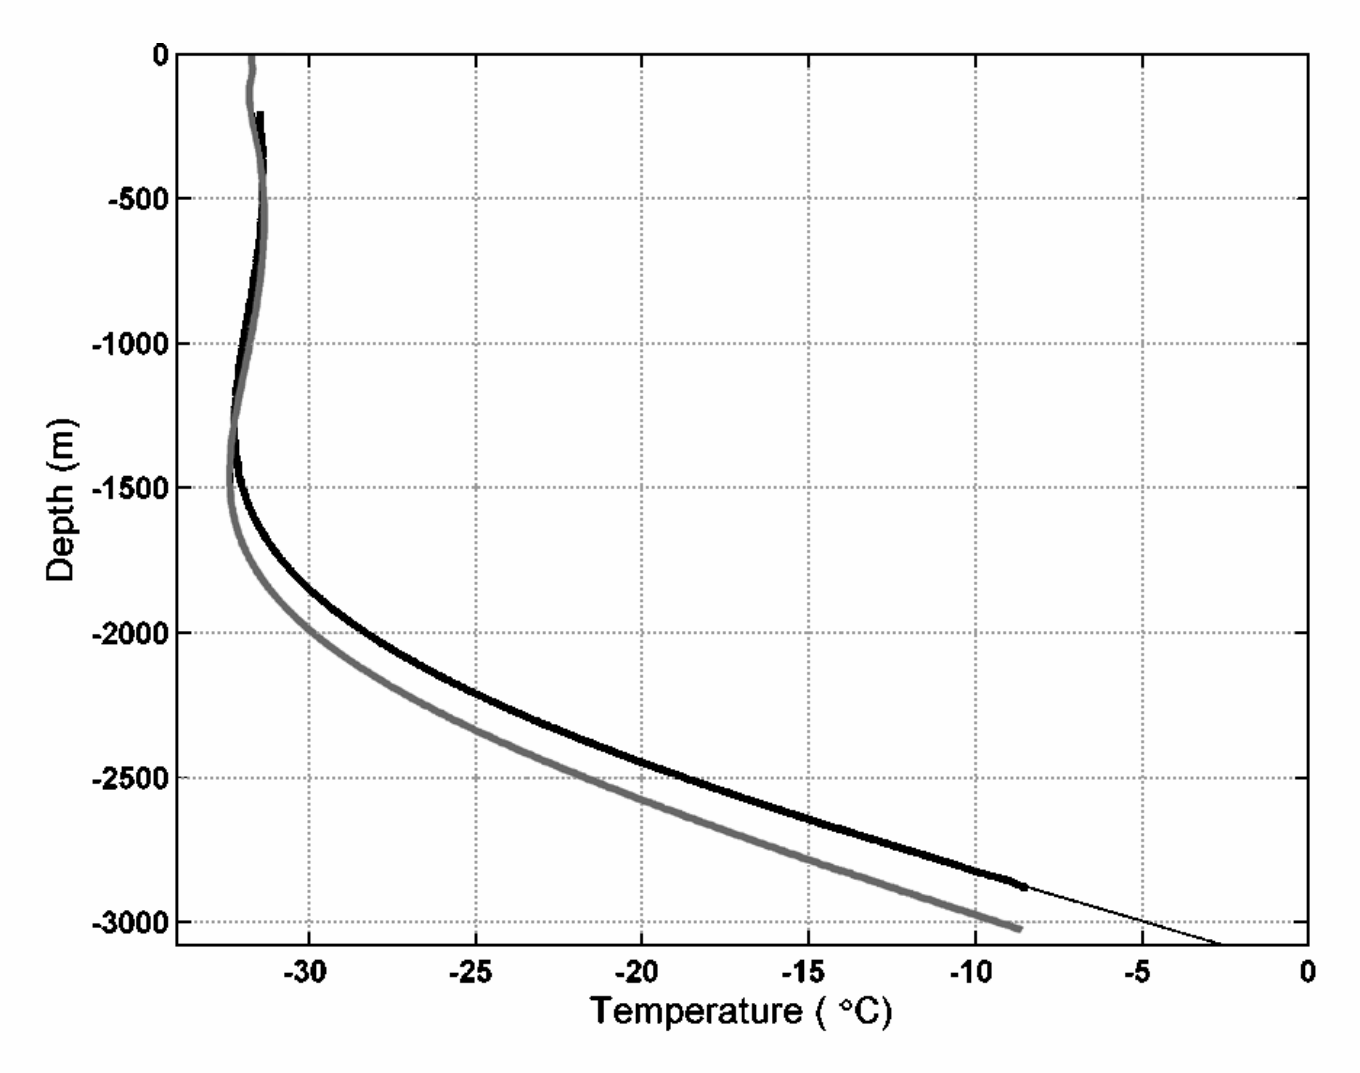
\includegraphics[width=.9\linewidth]{ngrip/dahl-jensen_2003_fig1.png}
\end{center}

\subsubsection{Thickness}
\label{sec:org592fae6}

\begin{itemize}
\item From \textcite{dahl-jensen_2003} (abstract)
\end{itemize}

\subsubsection{Location}
\label{sec:orgfa1805a}

\subsubsection{Velocity}
\label{sec:orgf460d20}
\clearpage
\subsection{Penny}
\label{sec:org944cfaf}
\begin{verbatim}
Name                                  | penny
Alternate name                        | Penny Ice Cap
Data source                           | WIC
Drill year(s)                         | 
Data year(s)                          | 1996
Longitude [°E]                        | -65.2
Latitude [°N]                         | 67.3
Approximate location name             | 
Location source                       | 
Ice thickness [m]                     | 176
Ice thickness year                    | 
Ice thickness source                  | Data file + WIC email (see also Fisher 1998)
Surface velocity [m yr^-1]            | 
Surface velocity year                 | 
Surface velocity source               | 
Measured from: Top, Bottom, Relative  | T
Depth of top measurement [m]          | 10.0
Depth of bottom measurement [m]       | 176.0
\end{verbatim}

\subsubsection{Temperature}
\label{sec:org20cb956}

\begin{itemize}
\item Data provided from Liam email: \href{msgid:AM0PR04MB6129F2DC55EE1ACDB5107ED5A2CC0@AM0PR04MB6129.eurprd04.prod.outlook.com}{Penny T profile?}
\end{itemize}

\begin{verbatim}
From: William Colgan
To: Ken Mankoff
Subject: Penny T profile?
Date: Wed 09 Dec 2020 03:17:20 AM PST
Attachments: [1]Penny 1996 borehole T profile.xlsx(303.9K)

Hey Ken – Here is the last of the Canadian Arctic Ice Caps. Penny! For the IceTemp database. The 1996 profile is to bedrock.

Penny site:
Latitude           N 67 deg 18'
Longitude        W 65 deg 12'

Fra: Christian Zdanowicz
Sendt: 2. december 2020 13:27
Til: William Colgan
Emne: RE: Prince of Wales - ice temperature?

So here you are (attachments). There were two T profiles measured through Penny ice cap,
one in the 1996 borehole, one in the 1998 borehole. I distrust the 1998 profile, because
it is likely that the termistor got stuck in the borehole, as the constant Ts below 140 m
suggest (see figure in the Excel spreadsheet). The T profile in the 1996 borehole, measured
in 1997, is more trustworthy. See attached paper (JGR 2012) for borehole locations.

David Fisher deserves the credit for all these data, I did not generate them. You can use
his Univ. of Ottawa affiliation: Department of Earth and Environmental Sciences, University
of Ottawa, Ottawa, Canada, K1N 6N5.
\end{verbatim}


\subsubsection{Thickness}
\label{sec:orgf831a95}

\begin{itemize}
\item From WIC email
\end{itemize}

\subsubsection{Location}
\label{sec:org4ce43cf}

\begin{itemize}
\item From WIC email
\end{itemize}

\subsubsection{Velocity}
\label{sec:orgea24c42}
\clearpage
\subsection{Prince of Wales}
\label{sec:org30f0537}
\begin{verbatim}
Name                                  | pow
Alternate name                        | Prince of Wales
Data source                           | WIC
Drill year(s)                         | 
Data year(s)                          | 2005-05-15
Longitude [°E]                        | -80.395
Latitude [°N]                         | 78.3897
Approximate location name             | 
Location source                       | 
Ice thickness [m]                     | 176
Ice thickness year                    | 
Ice thickness source                  | WIC
Surface velocity [m yr^-1]            | 
Surface velocity year                 | 
Surface velocity source               | 
Measured from: Top, Bottom, Relative  | T
Depth of top measurement [m]          | 10.0
Depth of bottom measurement [m]       | 176.0
\end{verbatim}

\subsubsection{Temperature}
\label{sec:org8aa1b43}

\begin{itemize}
\item Email from WIC: \href{msgid:AM0PR04MB61293648564AB69ACA6A02CBA2F30@AM0PR04MB6129.eurprd04.prod.outlook.com}{VS: Prince of Wales - ice temperature?}
\end{itemize}

\begin{verbatim}
From: William Colgan
To: Ken Mankoff
Subject: VS: Prince of Wales - ice temperature?
Date: Wed 02 Dec 2020 03:06:55 AM PST
Attachments: [1]PoW_T_profile.xlsx(20.2K)

Ken, Here is “Prince of Wales Icefield” on Ellesmere (“PoW”) for the IceTemp database. Full profile to ice bottom at 176 m.

Coordinates: N 78 deg 23.382, W 80 deg 23.700

Fra: Christian Zdanowicz
Sendt: 2. december 2020 10:48
Til: William Colgan
Emne: RE: Prince of Wales - ice temperature?

Here is what I have. Not much, unfortunately, but better than nothing. The
measurements were made on 15 May 2005, the day after the drill reached
bedrock. The borehole had been started on 3 May 2005, so surface air may have
circulated in the borehole for up to 10 days between start and end of drilling
(although borehole was closed with a lid between drilling days).

The measurements were done with Richard Brancker Research Ltd (RBR; now
RBR Global: https://rbr-global.com/) programmable probe model RBR TR-1050.
(manual attached, for reference). The coefficients of the quandratic calibration
equation that relates measured vs. certified temperature were -0.000251638,
0.00000239321E-06, and -0.000000063277540 (deg C).

The actual depths recorded are very approximate. This is the way I made the
measurements: I suspended the RBR temperature probe on a long string marked at
one-metre intervals. Because of the weight of the string itself, it was impossible
to guess "by feel" when the probe touched the bottom of the borehole. Instead, I
lowered the probe down to the 180 m mark, which is slightly deeper than the
borehole (~176 m). I then raised the probe 10 metres every hours. The probe was
programmed to take one reading every hour on the hour, and I raised the probe
about 5 minutes into the hour to allow 50 minutes at every level for the probe
to equilibrate with the ambient temperature.
\end{verbatim}


\subsubsection{Thickness}
\label{sec:orgb783cea}

\begin{itemize}
\item Email from WIC: \href{msgid:AM0PR04MB61293648564AB69ACA6A02CBA2F30@AM0PR04MB6129.eurprd04.prod.outlook.com}{VS: Prince of Wales - ice temperature?}
\end{itemize}

\subsubsection{Location}
\label{sec:orge47cc7b}

\begin{itemize}
\item Email from WIC: \href{msgid:AM0PR04MB61293648564AB69ACA6A02CBA2F30@AM0PR04MB6129.eurprd04.prod.outlook.com}{VS: Prince of Wales - ice temperature?}
\end{itemize}

\subsubsection{Velocity}
\label{sec:org677411d}
\clearpage
\subsection{Renland}
\label{sec:orgc95ea14}
\begin{verbatim}
Name                                  | renland
Alternate name                        | Renland
Data source                           | BMV
Drill year(s)                         | 
Data year(s)                          | 1988
Longitude [°E]                        | -26.73
Latitude [°N]                         | 71.27
Approximate location name             | 
Location source                       | Vinther (2008)
Ice thickness [m]                     | 324.4
Ice thickness year                    | 
Ice thickness source                  | Vinther, B. M., Clausen, H. B., Fisher, D. A., Koerner, R. M., Johnsen, S. J., Andersen, K. K., Dahl-Jensen, D., Rasmussen, S. O., Steffensen, J. P., Svensson, A. M.: Synchronizing ice cores from the Renland and Agassiz ice caps to the Greenland Ice Core Chronology , Journal of Geophysical Research 113(D8), American Geophysical Union (AGU), 4 2008 
Surface velocity [m yr^-1]            | 
Surface velocity year                 | 
Surface velocity source               | 
Measured from: Top, Bottom, Relative  | T
Depth of top measurement [m]          | 15.0
Depth of bottom measurement [m]       | 300.0
\end{verbatim}

\subsubsection{Temperature}
\label{sec:org913b98c}

\begin{itemize}
\item Mentioned in \textcite{vinther_2008}
\item As per email from Bo Vinther (\href{msgid:2033620922.1391238.1606871518421@titapp04}{SV: SV: Renland ice temperature profile?}),
\begin{itemize}
\item Surface velocity small
\item The position of the 1988 site is: 71.306N, 26.768W.
\item In 1988 the drill got stuck at 324.4m depth - radar measurements suggested a depth of some 321+/-5m \autocite{johnsen_1992}
\item Temperature provided as XLS attachment in email: \href{msgid:9d866df4f1bc4dd8aaa1216ad90406dc@nbi.ku.dk}{SV: Renland ice temperature profile?}
\end{itemize}
\item From \textcite{johnsen_1992}
\begin{itemize}
\item Basal temperature inferred to be -13 °C (p. 7)
\end{itemize}
\end{itemize}

\subsubsection{Thickness}
\label{sec:org4d449c3}

\begin{itemize}
\item Ice core length is 325 from \textcite{vinther_2008}.
\end{itemize}

\subsubsection{Location}
\label{sec:org8dc7fdb}

\begin{itemize}
\item From \textcite{vinther_2008}
\end{itemize}

\subsubsection{Velocity}
\label{sec:orgc7412ef}

\begin{itemize}
\item Likely small because drilling location near ice cap dome.
\end{itemize}
\clearpage
\subsection{Site II}
\label{sec:org9761280}
\begin{verbatim}
Name                                  | site_ii
Alternate name                        | Site II
Data source                           | Hansen, B. L., Landauer, J. K.: Some results of ice cap drill hole measurements, Union Geodesique et Geophysique Internationale. Association Internationale d'Hydrologie Scientifique 47, 313–317, 1958 
Drill year(s)                         | 1957 (Summer)
Data year(s)                          | 1958 (late June)
Longitude [°E]                        | -56.066667
Latitude [°N]                         | 76.983333
Approximate location name             | 
Location source                       | WIC Email
Ice thickness [m]                     | 1851
ice thickness year                    | 
Ice thickness source                  | BedMachine
Surface velocity [m yr^-1]            | 
Surface velocity year                 | 
Surface velocity source               | 
Measured from: Top, Bottom, Relative  | T
Depth of top measurement [m]          | 
Depth of bottom measurement [m]       | 
\end{verbatim}

\subsubsection{Temperature}
\label{sec:orga1ee5c3}

\begin{itemize}
\item Digitized from \textcite{hansen_1958} Figure 3:
\item WARNING: Depth reported in [ft] not [m].
\item WARNING: From text,
\end{itemize}

\begin{quote}
Final values will not be assigned to the 1958 data until the equipment
has been returned from Greenland and recalibrated.
\end{quote}

\begin{center}
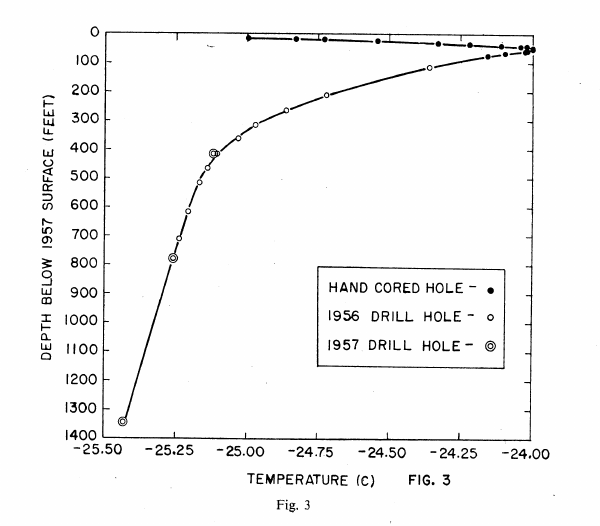
\includegraphics[width=.9\linewidth]{site_ii/hansen_1958_fig3.png}
\end{center}

\subsubsection{Thickness}
\label{sec:orgee94c28}

Link to email: \href{msgid:AM0PR04MB612902A1264CB3D0BA62E550A2C00@AM0PR04MB6129.eurprd04.prod.outlook.com}{Site II - temperature}

\begin{verbatim}
From: William Colgan
To: Ken Mankoff
Subject: Site II - temperature
Date: Sun 20 Dec 2020 11:37:39 PM PST

Here’s a temperature record for ”Site II” Greenland. This temperature
record only goes to 1346 ft, and total ice thickness is estimated in a
similar record at “6800 ft” (might be better to just interpolate from
BedMachine). This will be too shallow to extrapolate a basal
temperature, but I think it is a very useful ice temperature record in
general, similar to Camp VI.

Coordinates: 76°59′N 56°04′W

BedMachine has Site II as 1851 m total ice thickness. So lets go with
that, instead of “6800 ft”.
\end{verbatim}

\subsubsection{Location}
\label{sec:orgfbbfbb9}

Email from WIC (see above)

\subsubsection{Velocity}
\label{sec:org702943a}
\clearpage
\subsection{TD1}
\label{sec:orgdff9031}
\begin{verbatim}
Name                                  | td1
Alternate name                        | 
Data source                           | Unknown PDF: Shallow88II.pdf
Drill year(s)                         | 
Data year(s)                          | 1988-05-19
Longitude [°E]                        | -50.13
Latitude [°N]                         | 69.45
Approximate location name             | Paakitsoq
Location source                       | Unknown PDF: Shallow88II.pdf
Ice thickness [m]                     | 300
Ice thickness year                    | 
Ice thickness source                  | Unknown PDF: Shallow88II.pdf
Surface velocity [m yr^-1]            | 
Surface velocity year                 | 
Surface velocity source               | 
Measured from: Top, Bottom, Relative  | T
Depth of top measurement [m]          | 50.0
Depth of bottom measurement [m]       | 300.0
\end{verbatim}

\subsubsection{Temperature}
\label{sec:org3364fb7}

\begin{itemize}
\item See Shallow88II.pdf
\end{itemize}

\begin{verbatim}
From: Martin Luethi
To: Ken Mankoff
Subject: Re: TD5 from Thomsen 1991
Date: Thu 01 Oct 2020 02:27:19 PM PDT
Attachments: [1]thompson_profiles.zip(2.9M)

Ken Mankoff writes:
>> I'm looking for the source of the TD5 temperature profile you show in
>> your 2015 "Heat sources" paper in The Cryosphere. Your Figure 2 shows
>> TD5 and your text references Thomsen et al. 1991, and Thomsen &
>> Thorning, 1992.

Good questions. I probably don't have these papers, but I have some of
the profiles. I got them as paper copies from Heinz Blatter, and later
also some of them from Thomas Phillips. It's been a while, so I don't
have any details.

I also added some data from profiles I found in EGIG publications. 
\end{verbatim}

\subsubsection{Thickness}
\label{sec:org25a1acf}

\begin{itemize}
\item From PDF
\end{itemize}

\subsubsection{Location}
\label{sec:org1885109}

\begin{itemize}
\item From PDF
\end{itemize}

\subsubsection{Velocity}
\label{sec:orgb4e11c7}
\clearpage
\subsection{TD2}
\label{sec:org3e69e4c}
\begin{verbatim}
Name                                  | td2
Alternate name                        | 
Data source                           | Unknown PDF: See td1
Drill year(s)                         | 
Data year(s)                          | 1988-05-19
Longitude [°E]                        | -50.13
Latitude [°N]                         | 69.45
Approximate location name             | Paakitsoq
Location source                       | Unknown PDF: See td1
Ice thickness [m]                     | 470
Ice thickness year                    | 
Ice thickness source                  | Unknown PDF: See td1
Surface velocity [m yr^-1]            | 
Surface velocity year                 | 
Surface velocity source               | 
Measured from: Top, Bottom, Relative  | T
Depth of top measurement [m]          | 27.0
Depth of bottom measurement [m]       | 202.0
\end{verbatim}

\subsubsection{Temperature}
\label{sec:orgcb057fa}

\begin{itemize}
\item See td1 Shallow88II.pdf
\end{itemize}

\subsubsection{Thickness}
\label{sec:org0e77216}

\begin{itemize}
\item From PDF
\end{itemize}

\subsubsection{Location}
\label{sec:org5d47837}

\begin{itemize}
\item From PDF
\end{itemize}

\subsubsection{Velocity}
\label{sec:org5daeb82}
\clearpage
\subsection{TD3}
\label{sec:org0bc320e}
\begin{verbatim}
Name                                  | td3
Alternate name                        | 
Data source                           | Unknown PDF: See td1. Also Phillips (2010)
Drill year(s)                         | 
Data year(s)                          | 1988-08-18
Longitude [°E]                        | -50.1
Latitude [°N]                         | 69.483
Approximate location name             | Paakitsoq
Location source                       | Unknown PDF: See td1. Also Phillips (2010)
Ice thickness [m]                     | 350
Ice thickness year                    | 
Ice thickness source                  | Unknown PDF: See td1. Also Phillips (2010)
Surface velocity [m yr^-1]            | 
Surface velocity year                 | 
Surface velocity source               | 
Measured from: Top, Bottom, Relative  | T
Depth of top measurement [m]          | 20.0
Depth of bottom measurement [m]       | 350.0
\end{verbatim}

\subsubsection{Temperature}
\label{sec:orgcedb1a0}

\begin{itemize}
\item See td1 Shallow88II.pdf
\item Also see \textcite{phillips_2010} Figure 4.
\end{itemize}

\begin{center}
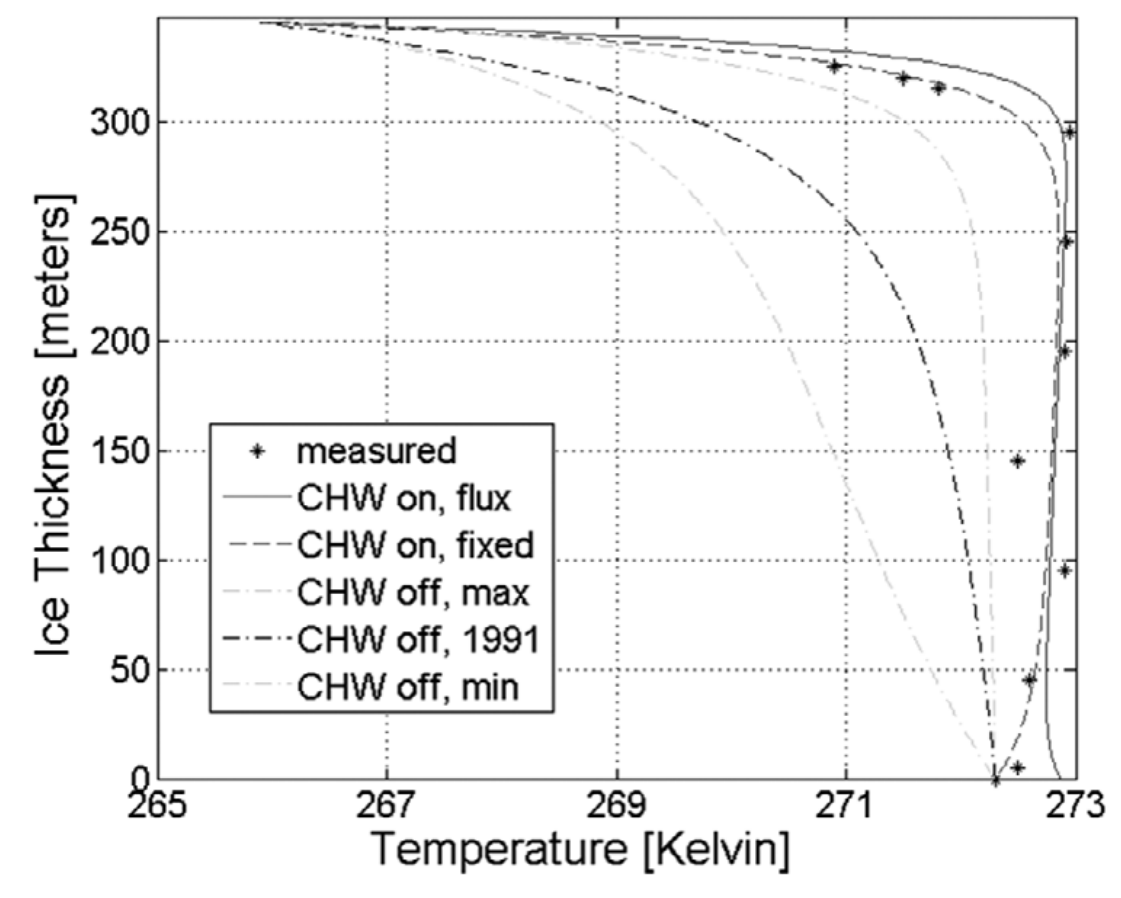
\includegraphics[width=.9\linewidth]{td3/phillips_2010_fig4.png}
\end{center}

\subsubsection{Thickness}
\label{sec:org9a575c8}

\begin{itemize}
\item From unknown PDF (see td1). Also reported in \textcite{phillips_2010}.
\end{itemize}

\subsubsection{Location}
\label{sec:org71bd2b2}

\begin{itemize}
\item From unknown PDF (see td1). Also reported in \textcite{phillips_2010}.
\end{itemize}

\subsubsection{Velocity}
\label{sec:org5cfdd7d}
\clearpage
\subsection{TD41}
\label{sec:org398b781}
\begin{verbatim}
Name                                  | td41
Alternate name                        | 
Data source                           | Unknown PDF: See td1
Drill year(s)                         | 
Data year(s)                          | 1991-11-05
Longitude [°E]                        | -49.683
Latitude [°N]                         | 69.533
Approximate location name             | Paakitsoq
Location source                       | Unknown PDF: See td1
Ice thickness [m]                     | >600
Ice thickness year                    | 
Ice thickness source                  | Unknown PDF: See td1
Surface velocity [m yr^-1]            | 
Surface velocity year                 | 
Surface velocity source               | 
Measured from: Top, Bottom, Relative  | T
Depth of top measurement [m]          | 5.0
Depth of bottom measurement [m]       | 495.0
\end{verbatim}

\subsubsection{Temperature}
\label{sec:org84e0af9}

\begin{itemize}
\item See td1 Shallow88II.pdf
\end{itemize}

\subsubsection{Thickness}
\label{sec:orgdcad4ee}

\begin{itemize}
\item From PDF
\end{itemize}

\subsubsection{Location}
\label{sec:orgb80930a}

\begin{itemize}
\item From PDF
\end{itemize}

\subsubsection{Velocity}
\label{sec:orgae0531b}
\clearpage
\subsection{TD42}
\label{sec:org56855d7}
\begin{verbatim}
Name                                  | td42
Alternate name                        | 
Data source                           | Unknown PDF: See td1
Drill year(s)                         | 
Data year(s)                          | 1991-08-28
Longitude [°E]                        | -49.683
Latitude [°N]                         | 69.533
Approximate location name             | Paakitsoq
Location source                       | Unknown PDF: See td1
Ice thickness [m]                     | >600
Ice thickness year                    | 
Ice thickness source                  | Unknown PDF: See td1
Surface velocity [m yr^-1]            | 
Surface velocity year                 | 
Surface velocity source               | 
Measured from: Top, Bottom, Relative  | T
Depth of top measurement [m]          | 3.0
Depth of bottom measurement [m]       | 493.0
\end{verbatim}

\subsubsection{Temperature}
\label{sec:org11f7681}

\begin{itemize}
\item See td1 Shallow88II.pdf
\end{itemize}

\subsubsection{Thickness}
\label{sec:org824ac54}

\begin{itemize}
\item From PDF
\end{itemize}

\subsubsection{Location}
\label{sec:org854f276}

\begin{itemize}
\item From PDF. Same location as td41. Unknown if same borehole.
\end{itemize}

\subsubsection{Velocity}
\label{sec:orgb03ee6c}
\clearpage
\subsection{TD51}
\label{sec:orgf7fb67e}
\begin{verbatim}
Name                                  | td51
Alternate name                        | 
Data source                           | Unknown PDF: See td1 and Lüthi (2015)
Drill year(s)                         | 
Data year(s)                          | 1990-06-09
Longitude [°E]                        | -49.3
Latitude [°N]                         | 69.566
Approximate location name             | Paakitsoq / Swiss Camp
Location source                       | Unknown PDF: See td1 and Lüthi (2015)
Ice thickness [m]                     | >600
Ice thickness year                    | 
Ice thickness source                  | Unknown PDF: See td1 and Lüthi (2015)
Surface velocity [m yr^-1]            | 
Surface velocity year                 | 
Surface velocity source               | 
Measured from: Top, Bottom, Relative  | T
Depth of top measurement [m]          | 5.0
Depth of bottom measurement [m]       | 600.0
\end{verbatim}

\subsubsection{Temperature}
\label{sec:org71cb8ea}

\begin{itemize}
\item See td1 Shallow88II.pdf and \textcite{luthi_2015}
\end{itemize}

\subsubsection{Thickness}
\label{sec:org459a59c}

\begin{itemize}
\item From PDF
\end{itemize}

\subsubsection{Location}
\label{sec:orgba8983e}

\begin{itemize}
\item From PDF
\end{itemize}

\subsubsection{Velocity}
\label{sec:orgbe3de60}
\clearpage
\subsection{TD52}
\label{sec:orgba5f2f8}
\begin{verbatim}
Name                                  | td52
Alternate name                        | 
Data source                           | Unknown PDF: See td1 and Lüthi (2015)
Drill year(s)                         | 
Data year(s)                          | 1991-05-25
Longitude [°E]                        | -49.3
Latitude [°N]                         | 69.566
Approximate location name             | Paakitsoq / Swiss Camp
Location source                       | Unknown PDF: See td1 and Lüthi (2015)
Ice thickness [m]                     | >600
Ice thickness year                    | 
Ice thickness source                  | Unknown PDF: See td1 and Lüthi (2015)
Surface velocity [m yr^-1]            | 
Surface velocity year                 | 
Surface velocity source               | 
Measured from: Top, Bottom, Relative  | T
Depth of top measurement [m]          | 5.0
Depth of bottom measurement [m]       | 600.0
\end{verbatim}

\subsubsection{Temperature}
\label{sec:orgeac3047}

\begin{itemize}
\item See td1 Shallow88II.pdf. Also shown in \textcite{luthi_2015}.
\end{itemize}

\subsubsection{Thickness}
\label{sec:org92c01c6}

\begin{itemize}
\item From PDF
\end{itemize}

\subsubsection{Location}
\label{sec:org7bce8a2}

\begin{itemize}
\item From PDF. Same as td51. Unknown if same borehole.
\end{itemize}

\subsubsection{Velocity}
\label{sec:orgeaf9998}
\clearpage
\subsection{Tuto Ramp}
\label{sec:orgdccf8a1}
\begin{verbatim}
Name                                   |  tuto_ramp
Alternate name                         |  Tuto Ramp
Data source                            |  Davis, RM: Approach roads, Greenland 1960–1964 , Technical Report 133. Corps of Engineers, Cold Regions Research & Engineering Laboratory , 1967 
Data year(s)                           |  1962 (August)
Depth of top measurement [m]           |  
Depth of bottom measurement [m]        |  
Drill year(s)                          |  
Longitude [°E]                         |  -68.287295
Latitude [°N]                          |  76.41133
Approximate location name              |  Thule Approach Road(?)
Location source                        |  
Ice thickness [m]                      |  48
Ice thickness year                     |  
Ice thickness source                   |  See data source
Surface velocity [m yr^-1]             |  1.0
Surface velocity year                  |  
Surface velocity source                |  WIC Email
Measured from: Top, Bottom, Relative   |  T(ish)
\end{verbatim}

\subsubsection{Temperature}
\label{sec:org40252a7}

\begin{itemize}
\item From \textcite{davis_1967} Figure 31.
\item Digitized only August 1962 profile
\end{itemize}

\begin{center}
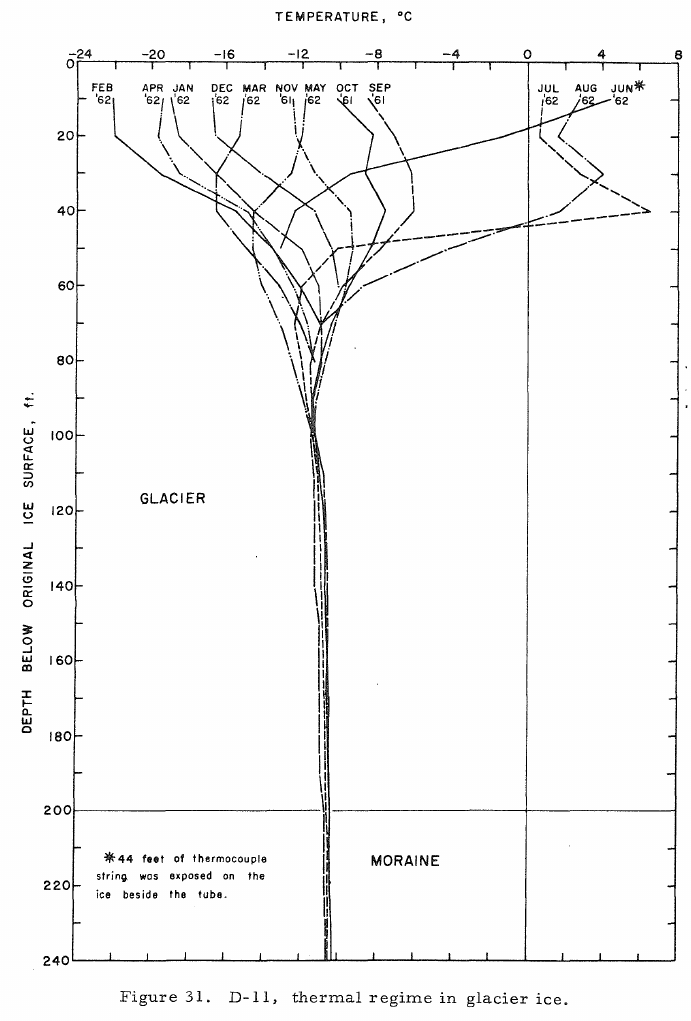
\includegraphics[width=.9\linewidth]{tuto_ramp/davis_1967_fig31.png}
\end{center}


\subsubsection{Thickness}
\label{sec:org73a04c0}

\begin{itemize}
\item Depth from text interpreted to mean that ice surface starts at 44 ft on cable and bottom is at 200 ft on cable -> thickness is 156 ft or 156*0.3048 = 47.5488
\end{itemize}

\subsubsection{Location}
\label{sec:orgddd86a0}

\begin{itemize}
\item Location comes from WIC digitizing some map and emailing me coordinates.
\end{itemize}

\subsubsection{Velocity}
\label{sec:org1b74e31}

\begin{itemize}
\item From WIC email
\end{itemize}

\clearpage
\section{Uncertainty}
\label{sec:orgc31ce1b}
Most of sources are digitized from graphics and the reported uncertainty is much less than the line-width relative to graph temperature scale. Therefore, we can ignore reported uncertainties. Instead, uncertainty can be estimated from the cases when the same data is presented multiple times, ideally in fundamentally different graphics in different publications, or comparing a digitized graphic to the original non-digitized source if it is available.

\subsection{NEEM}
\label{sec:org78ac859}

We have two sources for the NEEM data: 1) \textcite{macgregor_2015} relative depth profile graphic and 2) Data provided via email.

\begin{figure}[!h]
\centering
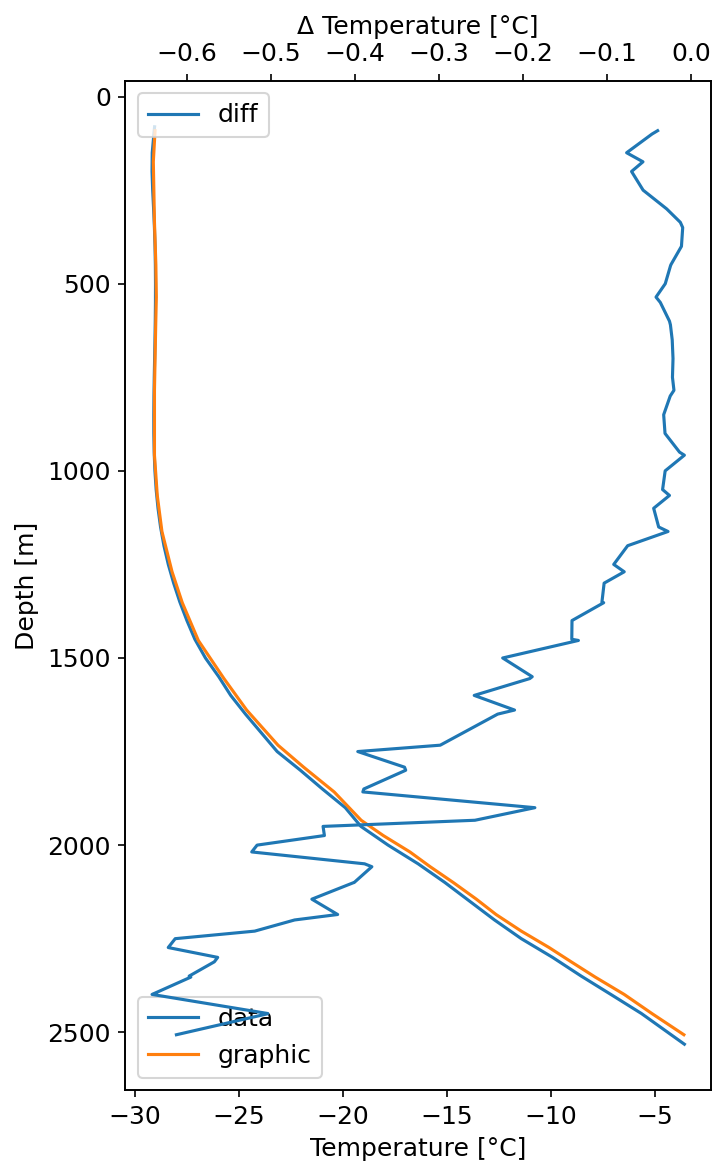
\includegraphics[width=0.5\textwidth]{./fig/neem_diff.png}
\caption{\label{fig:err_NEEM}Digitization error for the NEEM borehole temperature profile. This is likely a worst-case scenario for digitization error because the graphic used a wide line (uncertain temperature), only spanned \textasciitilde{}1/3 of the page, but spanned \textasciitilde{}30 ° of temperature (low resolution temperature), and had a highly compressed y-axis (uncertain depth)}
\end{figure}


\subsection{Agassiz}
\label{sec:org4500e6f}

The Agassiz boreholes were provided as data. By digitizing graphics from papers (e.g. \textcite{clarke_1987_wind}, we can find a measure of the digitization error.

\begin{figure}[!h]
\centering
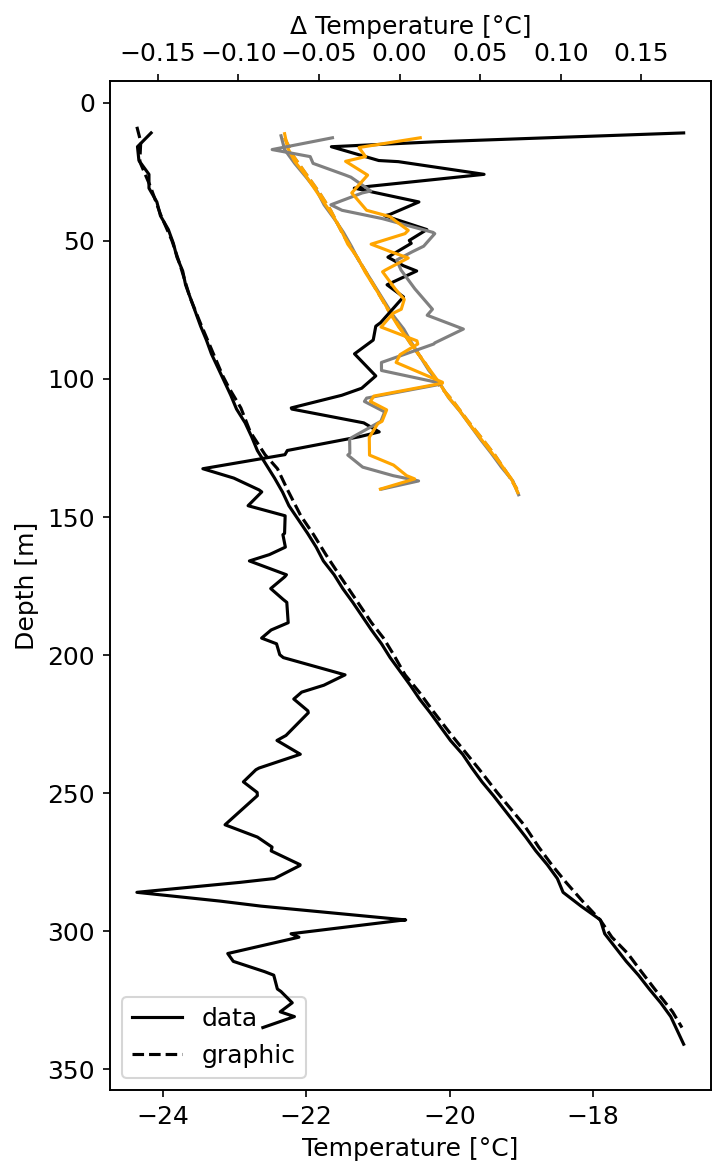
\includegraphics[width=0.5\textwidth]{./fig/agassiz_diff.png}
\caption{\label{fig:err_agassiz}Digitization error for Agassiz borehole temperature profiles. Black is A77 data, graphic, and difference (noisy line, top x-axis). Gray and orange are the difference between the \textcite{clarke_1987_wind} A79 profile from the graphic and the A79A and A79B data profiles, respectively.}
\end{figure}

\clearpage
\section{About This Document}
\label{sec:org5140f93}
This document is an Emacs Org Mode plain-text file with code and text embedded. If you are viewing:
\begin{itemize}
\item A DOC or PDF file, then it was generated by exporting from Org. Not all of the Org parts (code, results, comments, etc.) were exported. The Org source file is available upon request, and may be embedded in the PDF. Most non-Apple PDF viewers provide easy access to embedded or attached files.
\item A file with an \texttt{org} extension in something other than Emacs (e.g., in your browser on GitHub)l, then you are seeing the canonical version and the full source, but without any syntax highlighting, document structure, or the ability to execute the code blocks.
\item An \texttt{Org} file within Emacs, then this is the canonical version. You should be able to fully interact and reproduce the contents of this document, although it may require 3rd-party applications (Python, etc.) and a similar Emacs configuration. This is available upon request.
\end{itemize}

\clearpage
\section{References}
\label{sec:orgb18e392}
\printbibliography[heading=none]
\end{document}
